\documentclass[12pt,a4paper,oneside]{report}             % Single-side
%\documentclass[12pt,a4paper,twoside,openright]{report}  % Duplex

\usepackage{t1enc}
\usepackage[utf8]{inputenc}
\usepackage{amsmath}
\usepackage{amssymb}
\usepackage{enumerate}
\usepackage[thmmarks]{ntheorem}
\usepackage{graphics}
\usepackage{epsfig}
\usepackage{listings}
\usepackage{color}
%\usepackage{fancyhdr}
\usepackage{lastpage}
\usepackage{anysize}
\usepackage[hungarian]{babel}
\usepackage{sectsty}
\usepackage{setspace}  % Ettol a tablazatok, abrak, labjegyzetek maradnak 1-es sorkozzel!
\usepackage[hang]{caption}
\usepackage[unicode]{hyperref}

\usepackage[T1]{fontenc}
\usepackage{lmodern}
\usepackage{listings} % code samples
\usepackage{courier}
\usepackage{bm} % bold faced letters in math mode

%--------------------------------------------------------------------------------------
% Main variables
%--------------------------------------------------------------------------------------
\newcommand{\vikszerzo}{Thaler Benedek}
\newcommand{\vikkonzulens}{Rajacsics Tamás}
\newcommand{\vikcim}{Dinamikus kódanalízisen alapuló prediktív holtpontdetektálás}
\newcommand{\viktanszek}{Automatizálási és Alkalmazott Informatikai Tanszék}
\newcommand{\vikdoktipus}{Szakdolgozat}
\newcommand{\vikdepartmentr}{Thaler Benedek}

%--------------------------------------------------------------------------------------
% Page layout setup
%--------------------------------------------------------------------------------------
% we need to redefine the pagestyle plain
% another possibility is to use the body of this command without \fancypagestyle
% and use \pagestyle{fancy} but in that case the special pages
% (like the ToC, the References, and the Chapter pages)remain in plane style

\pagestyle{plain}
%\setlength{\parindent}{0pt} % áttekinthetõbb, angol nyelvû dokumentumokban jellemzõ
%\setlength{\parskip}{8pt plus 3pt minus 3pt} % áttekinthetõbb, angol nyelvû dokumentumokban jellemzõ
\setlength{\parindent}{12pt} % magyar nyelvû dokumentumokban jellemzõ
\setlength{\parskip}{0pt}    % magyar nyelvû dokumentumokban jellemzõ

\marginsize{35mm}{25mm}{15mm}{15mm} % anysize package
\setcounter{secnumdepth}{0}
\sectionfont{\large\upshape\bfseries}
\setcounter{secnumdepth}{2}
\singlespacing
\frenchspacing

%--------------------------------------------------------------------------------------
%	Setup hyperref package
%--------------------------------------------------------------------------------------
\hypersetup{
%    bookmarks=true,            % show bookmarks bar?
%    unicode=false,             % non-Latin characters in Acrobats bookmarks
    pdftitle={\vikcim},        % title
    pdfauthor={\vikszerzo},    % author
    pdfsubject={\vikdoktipus}, % subject of the document
    pdfcreator={\vikszerzo},   % creator of the document
    pdfproducer={Producer},    % producer of the document
    pdfkeywords={keywords},    % list of keywords
    pdfnewwindow=true,         % links in new window
    colorlinks=true,           % false: boxed links; true: colored links
    linkcolor=black,           % color of internal links
    citecolor=black,           % color of links to bibliography
    filecolor=black,           % color of file links
    urlcolor=black             % color of external links
}

%--------------------------------------------------------------------------------------
% Set up listings
%--------------------------------------------------------------------------------------
\lstset{
	basicstyle=\scriptsize\ttfamily, % print whole listing small
	keywordstyle=\color{black}\bfseries, % bold black keywords
	identifierstyle=, 					% nothing happens
	commentstyle=\color{black}, % black comments
	showstringspaces=false,     % no special string spaces
	aboveskip=3pt,
	belowskip=3pt,
	columns=fixed,
	backgroundcolor=\color{lightgray},
} 		
\def\lstlistingname{lista}	

%--------------------------------------------------------------------------------------
%	Some new commands and declarations
%--------------------------------------------------------------------------------------
\newcommand{\code}[1]{{\upshape\ttfamily\scriptsize\indent #1}}

% define references
\newcommand{\figref}[1]{\ref{fig:#1}.}
\renewcommand{\eqref}[1]{(\ref{eq:#1})}
\newcommand{\listref}[1]{\ref{listing:#1}.}
\newcommand{\sectref}[1]{\ref{sect:#1}}
\newcommand{\tabref}[1]{\ref{tab:#1}.}

\DeclareMathOperator*{\argmax}{arg\,max}
%\DeclareMathOperator*[1]{\floor}{arg\,max}
\DeclareMathOperator{\sign}{sgn}
\DeclareMathOperator{\rot}{rot}
\definecolor{lightgray}{rgb}{0.95,0.95,0.95}

% setup listing macro
\newcommand{\includecpp}[3]{
    \medskip    
    \lstset{
        basicstyle=\footnotesize\ttfamily
    }    
        \lstinputlisting[language=C++, firstline=#2, lastline=#3]{sources/#1.cpp}
    \medskip
}

\author{\vikszerzo}
\title{\viktitle}
\includeonly{
	project,% feladatkiiras
	titlepage,% cimoldal
	declaration,% nyilatkozat
	abstract,% kivonat
	introduction,% bevezeto
	chapter1,% elmelet
	chapter2,% megvalositas
	acknowledgement, %koszonet
}
%--------------------------------------------------------------------------------------
%	Setup captions
%--------------------------------------------------------------------------------------
\captionsetup[figure]{
%labelsep=none,
%font={footnotesize,it},
%justification=justified,
width=.75\textwidth,
aboveskip=10pt}

\renewcommand{\captionlabelfont}{\small\bf}
\renewcommand{\captionfont}{\footnotesize\it}

%--------------------------------------------------------------------------------------
% Table of contents and the main text
%--------------------------------------------------------------------------------------
\begin{document}
\singlespacing
%--------------------------------------------------------------------------------------
% Feladatkiiras (a tanszeken atveheto, kinyomtatott valtozat)
%--------------------------------------------------------------------------------------
\clearpage
\thispagestyle{empty} % hide page number
\begin{center}
\large
\textbf{FELADATKIÍRÁS}\\
\end{center}

A feladatkiírást a tanszéki adminisztrációban lehet átvenni, és a leadott munkába eredeti, tanszéki pecséttel ellátott és a tanszékvezető által aláírt lapot kell belefűzni (ezen oldal \emph{helyett}). Az elektronikusan feltöltött dolgozatban már nem kell beleszerkeszteni ezt a feladatkiírást.





\pagenumbering{arabic}
\onehalfspacing

\hypersetup{pageanchor=false}


%--------------------------------------------------------------------------------------
%	The title page
%--------------------------------------------------------------------------------------
\begin{titlepage}
\begin{center}


\includegraphics[width=60mm,keepaspectratio]{figures/BMElogo.png}\\
\vspace{0.3cm}
\textbf{Budapesti Műszaki és Gazdaságtudományi Egyetem}\\
\textmd{Villamosmérnöki és Informatikai Kar}\\
\textmd{\viktanszek}\\[5cm]

\vspace{0.4cm}
{\huge \bfseries \vikcim}\\[0.8cm]
\vspace{0.5cm}
\textsc{\Large \vikdoktipus}\\[4cm]

\begin{tabular}{cc}
 \makebox[7cm]{\emph{Készítette}} & \makebox[7cm]{\emph{Konzulens}} \\
 \makebox[7cm]{\vikszerzo} & \makebox[7cm]{\vikkonzulens}
\end{tabular}

\vfill
{\large \today}

\end{center}
\thispagestyle{empty}
\end{titlepage}




\tableofcontents\vfill
\addtocontents{toc}{\protect\thispagestyle{empty}}
\thispagestyle{empty}
\cleardoublepage

\hypersetup{pageanchor=true}

\pagestyle{plain}
%--------------------------------------------------------------------------------------
% Nyilatkozat
%--------------------------------------------------------------------------------------
\begin{center}
\large
\textbf{HALLGATÓI NYILATKOZAT}\\
\end{center}

Alulírott \emph{\vikszerzo}, szigorló hallgató kijelentem, hogy ezt a szakdolgozatot meg nem engedett segítség nélkül, saját magam készítettem, csak a megadott forrásokat (szakirodalom, eszközök stb.) használtam fel. Minden olyan részt, melyet szó szerint, vagy azonos értelemben, de átfogalmazva más forrásból átvettem, egyértelműen, a forrás megadásával megjelöltem.

Hozzájárulok, hogy a jelen munkám alapadatait (szerző(k), cím, angol és magyar nyelvű tartalmi kivonat, készítés éve, konzulens(ek) neve) a BME VIK nyilvánosan hozzáférhető elektronikus formában, a munka teljes szövegét pedig az egyetem belső hálózatán keresztül (vagy autentikált felhasználók számára) közzétegye. Kijelentem, hogy a benyújtott munka és annak elektronikus verziója megegyezik. Dékáni engedéllyel titkosított diplomatervek esetén a dolgozat szövege csak 3 év eltelte után válik hozzáférhetővé.

\begin{flushleft}
\vspace*{1cm}
Budapest, \today
\end{flushleft}

\begin{flushright}
 \vspace*{1cm}
 \makebox[7cm]{\rule{6cm}{.4pt}}\\
 \makebox[7cm]{\emph{\vikszerzo}}\\
 \makebox[7cm]{hallgató}
\end{flushright}
\thispagestyle{empty}

\vfill
\clearpage
\thispagestyle{empty} % an empty page


%----------------------------------------------------------------------------
% Abstract in hungarian
%----------------------------------------------------------------------------
\chapter*{Kivonat}
\addcontentsline{toc}{chapter}{Kivonat}

A konkurens végrehajásra képes rendszerek terjedése felgyorsította a párhuzamosságot támogató szoftver architektúrák és algoritmusok fejlődését. A parallel rendszerek tervezése komoly kihívást jelent, a hibásan kialakított vagy implementált alkalmazások karbantartása költséges és megterhelő feladat az üzemeltető számára. A dolgozat az előforduló problémák jellegének részletes tárgyalása mellett számos technikát ismertet, melyekkel ezek elkerülhetőek. Az ismertetett technikák kihasználják a \cite{C++11} szabvány számos újdonságát; a konkurenciát támogató szinkronizációs primitíveket, a tranzakcionális memóriát kihasználó atomi memória objektumokat és a \emph{move} szemantikát.

A második fejezet bemutat egy dinamikus kódanalízisen alapuló alkalmazást, mely hatékonyan képes előre jelezni egy rendszer holtpontjait, olyan kritikus helyzetekben is megoldást nyújtva, ahol más megoldások implementálása nagyon költséges lenne, az átalakítással járó fejlesztési erőfeszítések vagy a teljesítményromlás miatt.
\vfill

%----------------------------------------------------------------------------
% Abstract in english
%----------------------------------------------------------------------------
\chapter*{Abstract}
\addcontentsline{toc}{chapter}{Abstract}

The widespread of multicore processor architectures facilitate and speeds up the development of concurrent software architectures and algorithms. Being a rather tough challenge the design of such systems, failure to design or implement a concurrent application often implies serious maintenance costs later. This thesis describes the common pitfalls like race condition and deadlock and enumerates several solution which counteract and prevent them. The solutions make use of the brand new and highly anticipated features of the \cite{C++11} standard, like the synchronization primitives supporting concurrency, the atomic memory objects and methods which exposes the interesting capabilities of transactional memory and the move semantics.

The second chapter introduces an analyzer tool based on dynamic code analysis which is able to predict the deadlocks of a system. This tool successfully provides diagnostics even in cases where the other standard solutions would require excess refactoring or would cause significant performance degradation.
\vfill 


%----------------------------------------------------------------------------
\chapter*{Bevezető}
\addcontentsline{toc}{chapter}{Bevezető}
%----------------------------------------------------------------------------

% Mik azok a paralell rendszerek, miért fontosak (manapság), milyen problémák merülnek fel, ezekre eddig milyen válaszok érkeztek. A felmerülő témák közül mivel foglalkozik a dolgozat, egyes fejezetek mit járnak körbe.

Napjainkban már a középkategóriás okostelefonok is gyakran négymagos processzort tartalmaznak. A korábban csak a szuperszámítógépek luxusának tekintett konkurens architektúrák már a mindennapok szerves részét képezik. A több végrehajtó egységgel rendelkező platformok erőforrásait csak a jól skálázódó többszálú programok képesek megfelelően kihasználni. A párhuzamos szemlélet elsajátítása nem egyszerű, a megváltozott eszköz architektúra új algoritmusokat és szoftver architektúrákat igényel. Az új megoldások új típusú problémákat okoznak, melyek közül a stabilitás és megbízhatóság szempontjából különösen veszélyesek a nehezen reprodukálható és felderíthető versenyhelyzetek (\emph{race condition}) és holtpontok (\emph{deadlock}).

A dolgozat első fejezete egy elméleti áttekintést nyújt a paralell rendszerekről, a konkurens megoldások bevezetésétől várható tejlesítménynövekedésről, a modern operációs rendszereken elérhető szinkronizációs primitívekről, azoknak hardveres hátteréről és a gyakran alkalmazott optimalizációkról. A fejezet ezután a holtpont jelenség tárgyalását követően 6 technikát mutat be, melyek alkalmazásával különböző kompromisszumok mellett a holtpont elkerülhető. Az egyes megoldások összegzése részletezi az alkalmazhatóság korlátait, a várható előnyöket és hátrányokat. Az összefoglaló rámutat arra, hogy létezik elvárások olyan halmaza, melyet a bemutatott holtpont-megelőzési és -elkerülési technikák nem képesek kielégíteni.

A második fejezet bemutat egy olyan szoftvert, mely képes az előzőleg megoldatlan kérdéseket megválaszolni. A dinamikus kódanalízisen alapuló elemző lehetővé teszi egy rendszerben megtalálható holtpont lehetőségek felderítését és előrejelezését, nem téve szükségessé a holtpont bekövetkezését. A részletesen tárgyalt optimalizációknak köszönhetően lehetővé válik nagy áteresztő képességű (\emph{high throughput}) alkalmazások hatékony elemzése. A fejezet végül betekintést nyújt a fejlesztési tervekbe is.

%----------------------------------------------------------------------------
\chapter{Elméleti áttekintés}
%----------------------------------------------------------------------------

%----------------------------------------------------------------------------
\section{Paralell rendszerek}
%----------------------------------------------------------------------------

A félvezető alapú processzorok tranzisztorszáma hozzávetőlegesen megjelenésük óta \cite{Moore} törvényének megfelelően minden két évben megduplázódik. Az exponenciális növekedés lehetővé teszi a processzorok órajelének felskálázását, nagyobb memóriák előállítását, sőt, még a digitális kamerák szenzorainak pixelméretét is érinti. A jelenlegi tranzisztor koncepció és gyártástechnológia nem enged meg atomi méretnél kisebb tranzisztorokat, így a hagyományos tranzisztorok exponenciális növekedésben idővel letörés várható, azonban a processzorok órajelének növekedését már most egy sokkal súlyosabb akadály hátráltatja: a rengeteg, kis helyre zsúfolt félvezető eszköz hőterhelése olyan nagy, hogy az eszköz önmagát megrongálja. A jelenség miatt a processzor órajel növekedés mértéke a 2000-es évek elején csökkenésnek indult \cite{CMOS-VLSI}. A technikai fejlődés folytonossága érdekében a félvezetőgyártók -- a tranzisztorok zsúfoltságát csillapítandó -- egy processzorba több végrehajtó egységet (\emph{magot}) kezdek integrálni, melyek párhuzamosan dolgozva képesek egységnyi idő alatt több utasítást végrehajtani, a hőterhelés túlzott koncentrálása nélkül, ezzel megnyitva egy új korszakot a modern szoftverfejlesztésben.

    A többmagos rendszerek megjelenése egy sor új lehetőséget és kihívást állít a szoftverfejlesztők elé, akik ki akarják használni a konkurens rendszerek képességeit, azaz több szálat, folyamatot kívánnak párhuzamosan utilizálni. A piaci lehetőség elsősorban abban rejlik, hogy az a szoftver, ami képes elosztottan működni, és így teljesítménye a végrehajtóegységek számának növekedésével jól skálázódik, szignifikánsan hatékonyabb, mint azok, amik nem képesek erre. Az ebben az értelemben hatékony rendszerek fejlesztési költségeinek megnövekedését a konkurens rendszerek természetéből fakadók kihívások okozzák. (Megjegyzendő, hogy a többszálú alkalmazások megjelenése megelőzte a többmagos processzorok elterjedését, utóbbi csak növelte a konkurens természet jelentőségét.)
    
    % nem determinisztikussag 
    Az egyik legfontosabb különbség, amivel a programozó egy konkruens rendszer fejlesztése során szembesül, hogy az utasítások végrehajtásának sorrendje nem determinisztikus a többszálúság végett. Ennek következtében nem elég a program működésével \emph{nagyjából} tisztában lenni, nem lehet néhány tesztesetet lefuttatva megbizonyosodni a funkcionalitás helyességéről: bármikor előfordulhat, hogy a teszteset futtatásakor éppen kedvező volt a szálak ütemezése, és így a végeredmény értelmében helyes működés volt megfigyelhető, azonban a program hibás, más ütemezés, időzítés esetén viszont ennek megfelelően hibás eredményre fog jutni. A párhuzamosan futó szálak helyes működésének biztosítását és a szinkronizációs lehetőségeket az \ref{sec:communication_of_parallel_systems} szakasz tárgyalja.
    
    % parhuzamosithato reszek felderitese, 
    Az előbbi, leginkább technikai nehézségen megoldandó problémát jelent egy program komponenseinek párhuzamosítása. A fejlesztőnek azonosítania kell azokat a részeket, amelyek képesek egymástól függetlenül működni, nem támaszkodnak a másik eredményeire, így az egyes tevékenységek külön szálakon végezhetőek, akár egy időben is. Az ilyen egyszerű módon párhuzamosítható feladatokat nevezzük triviálisan párhuzamosíthatónak. Triviálisan párhuzamosítható algoritmus a mátrixszorzás algoritmusa: $\bm A \cdot \bm B = \bm C$ esetén $\bm C_{i, j}$ értéke csak $\bm A_i$ és $\bm B_j$ függvénye. A jól párhuzamosítható algoritmusok fejlesztése aktív kutatási terület.
    
    Más esetekben előfordulhat, hogy két komponens függ egymástól, működésük mégis átlapolható: ha $B$ feladat $i+1.$ iterációja csak $A$ feladat $i.$ iterációjától függ, a két feladat $i+1.$ iterációja futhat párhuzamosan. Egy ilyen típusú feladatra példa lehet egy olyan rendszer, ami szövegfájlokat dolgoz fel és az eredményeit egy adatbázisba írja. A fenti definíciónál maradva itt $A$-val jelölhetjük a fájl egy nagyobb részének beolvasását és feldolgozását, míg $B$-vel az adatbázis írását. Amíg $A$ olvassa a fájlt és a lemezművelet miatt blokkolódik, $B$ kiírhatja az előző számítás eredményeit, fordítva pedig amikor $B$ az adatbázisművelet befejezésére vár, $A$ olvashatja és feldolgozhatja a bemeneti fájl következő darabját. Az ilyen típusú szétcsatolások felderítése és kiaknázása jelenti a szoftverek párhuzamosításának elsődleges célpontját.
    
    Léteznek továbbá olyan algoritmikus problémák, amelyek szándékosan úgy lettek megalkotva, hogy ne lehessen őket disztributálni. A \cite{bcrypt} kriptográfiai algoritmus a bemenetén specifikált értékkel arányosan sok iterációt végez, továbbá minden egyes iteráció támaszkodik az előző eredményére. Ebben az esetben a motiváció az elosztott és párhuzamos rendszerek által végzett kódtörés elleni védelem elősegítése.
    
    % Itanium
    Felmerül a kérdés, hogyha a teljesítménynövekedés ennyire egyértelmű, miért nem végzi el a párhuzamosítható részek keresését a fordító program vagy a processzor, ahogy teszik azt számos más optimalizáció esetében. Mivel a processzor nem ismerheti a végrehajtandó utasítások szemantikáját, magas szintű párhuzamosíthatóság felderítésére aligha van lehetőség. Ellenben a fordítóprogram által párhuzamosított program végrehajtását támogató utasításkészletek léteznek, például a \cite{VLIW}, vagy az Intel Itanium processzorcsalád alapja, az \cite{EPIC}. Az ilyen architektúrájú processzorok lényegében több párhuzamos csővezetékkel (\emph{pipeline}) rendelkeznek, melyekben képesek párhuzamos utasításvégrehajtásra. A megközelítés hátránya, hogy a hatékony működéshez megfelelő heurisztikákat alkalmazó fordítókra lenne szükség, azonban ezek a mai napig kutatás tárgyát képezik.
    
    A párhuzamosított programokat futtatni képes konkurens rendszerek sem jelentenek tetszőleges mértékben skálázható teljesítménynövekedést. \cite{Amdahl} törvénye kimondja, hogyha a programunknak csupán $B$ hányada nem párhuzamosítható (márpedig ilyen hányad napjaink programjainak természetéből fakadóan mindig akad, pl.: futtatókörnyezet inicializáció, felhasználói interakcióra várakozás, adatbázis és hálózati műveletek, stb.), és ezt a programot egy $n$ szálat párhuzamosan futtatni képes processzoron futtatjuk, akkor a végrehajtáshoz szükséges idő arányos lesz $T(n)$-nel:
    
    \begin{equation}
        T(n) = T(1)\big(B+\frac{1}{n}(1-B)\big)
    \medskip
    \end{equation}
%    
    Ebből következően az elméleti sebességnövekedés adott rendszeren $S(n)$:
    
    \begin{equation} \label{eq:amdahl}
        S(n) = \frac{T(1)}{T(n)} = \frac{1}{B+\frac{1}{n}(1-B)}
    \medskip
    \end{equation}
%
%   \eqref{eq:amdahl} fails to ref for some reason.
    Az $(1.2)$ egyenletbe $B = 0.05$ értéket helyettesítve $\lim\limits_{n \rightarrow \infty}{S(n)}$ értéke $20$-nak adódik, avagy ha programunknak csak $5\%$-a nem párhuzamosítható, hiába futtatjuk a fennmaradó részét akár végtelen sok feldolgozó egységgel rendelkező architektúrán, csupán hússzoros teljesítménynövekedést érhetünk el.

    \subsection{Paralell rendszerek kommunikációja} 
    \label{sec:communication_of_parallel_systems} 
        
    Egy elosztott, konkurens rendszerben szükség lehet az egyes ágensek között információcsere biztosítására. Például a korábban említett átlapolt esetben a beolvasást és feldolgozást végző ágensnek értesíteni kell az adatbázisműveleteket végzőt, hogy a következő szelet processzálása megtörtént, az kész az adatbáziba írásra. Ekkor az eredményközlést és a kérdéses adat átadását úgy kell megvalósítani, hogy a jelzési folyamat során egyik ágens se érzékelhessen inkonzisztens állapotot a rendszerben -- a változtatásokat atomi módon kell végrehajtani.
        
    Máskor több ágens írhatja és olvashatja ugyan azt a fájlt (vagy más erőforrást), ekkor meg kell oldani a kérések sorosítását, mivel valódi párhuzamos hozzáférés esetén a fájl tartalma korrumpálódhatna -- az ágensek kölcsönös kizárását kell biztosítani.
        
    % critical section
    Ezek a problémák megoldhatóak akkor, ha biztosítható az ágensek számára a kritikus szakaszok egy időben kizárólagos végrehajtása, azaz egy adott szakaszban egyszerre csak egy ágens tartózkodhat. Kritikus szakasz elméleti vázlata a következő lehet: Minden szakasz jellemzője egy zár, amit az ágensek bezárhatnak, kinyithatnak és ellenőrizhetik az állapotát. Ekkor a kritikusz szakasz végrehajtása a következő:
        
    \begin{enumerate}
        \item Az ágens ellenőrzi, hogy a zár nyitva van-e. Ha nem, vár, majd újra próbálkozik.
        \item Ha nyitva találta a zárat, bezárja azt, ezzel jelezve belépését a kritikus szakaszba.
        \item Végrehatja a védendő utasításokat.
        \item Feloldja a zárat, ezzel kilépve a kritikus szakaszból, engedélyezve más ágensek számára a belépést.
    \end{enumerate}
%
    A továbbiakban tekintsünk egy folyamatot, mint konkurens rendszert, amelyben az ütemezett szálak az ágensek. A következő megállapítások általánosíthatóak elosztott rendszerekre. A fenti lépéssorozat naív (és így hibás) implementációja a következő:
    
    \includecpp{criticalsec-wrong}{3}{23}
        
    A fenti megoldás hibája, hogy amennyiben a \texttt{startCritical} metódust végrehajtó szál a \texttt{while} ciklusból való kilépés után elveszti a futási jogát, egy másik szál vele párhuzamosan zárolhatja ugyan azt a zárat, így amikor az előbbi szál újra ütemezésre kerül, egyszerre többen tartózkodhatnak azonos kritikus szakaszban. Valódi párhuzamosságot támogató architektúrán a hibás működés az ütemezéstől függetlenül is előfordulhat, ennek esélyét pedig a különböző végrehajtási egységek dedikált gyorsítótára csak növeli. A probléma felmerülhet egészen egyszerű beágyazott rendszerek esetén is, ahol a végrehajtás szigorúan egy szálon történik és csak egy folyamat van ütemezve, mivel megszakítás (\emph{interrupt}) bármelyik pillanatban érkezhet, így előidézheti a fent leírt jelenséget. Egyes egyszerű példákban megoldás lehet a megszakítások teljes letiltása, az esetek többségében azonban robosztusabb megoldásra van szükség.
    
    A probléma érdekessége, hogy a megoldáshoz hardware oldali támogatás elengedhetetlen. Mivel a zár ellenőrzését és zárolását atomi módon kell megtenni, szükség van arra, hogy az architektúra utasításkészlete ezt egy atomi utasítás formájában megvalósítsa. Ilyen utasítás lehet a \texttt{TSL} (\emph{Test and Set Lock}) vagy a \texttt{CAS} (\emph{Compare And Exchange}). Előbbi az egyik operandusának értékét a másik operandus által mutatott helyre írja, miután a felülírandó értéket egy maghatározott helyre mentette. A viselkedés felhasználható tevékeny várakozás megvalósítására: a zárolást végrehajtó ágens addig próbálja a zárt állapotnak megfelelő értéket a zár által mutatott címre írni, amíg az előző állapot nyitottnak nem adódik -- ekkor biztos lehet benne, hogy a zár az ellenőrzés pillanatában nyitva volt és azonos pillanatban (utasításban) általa zárolásra került.
    
    % CAS
    A \texttt{CAS} utasítás -- megvalósítástól függően -- összehasonlítja egyik operandusát egy regiszter értékével és azt egyezés esetén felülírja a másik operandussal. Amennyiben az összehasonlítás különbséget mutat, az első operandust érintetlenül hagyja és a sikertelenséget jelzi, például a \emph{zero flag} törlésével\footnote{http://courses.engr.illinois.edu/ECE390/archive/spr2002/books/labmanual/inst-ref-cmpxchg.html}. A megközelítés előnye, hogy versengés esetén nem történik memória írás, így elkerülhető a felesleges szinkronizáció. Napjaink konkurenciát támogató megoldásainak többsége a \texttt{CAS} utasításon alapul és minden jelentős platformon támogatott \cite{DiceEtAl}, a korábbi hibás konstrukciónak egy javított változata \texttt{CAS} használatával a következő lehet:
    
    \includecpp{criticalsec-cas}{6}{15}
    
    A \texttt{compare\_exchange\_weak} metódus első argumentumát hasonlítja össze az atomi objektum értékével, egyezés esetén azt a második paraméter értékével írja felül. Az összehasonlítás eredményét visszatérési értékével jelzi. Az atomi utasításokon alapulú konkurenciát támogató struktúrák az \ref{seq:lockfree} szakaszban kerülnek ismertetésre.
    
    A fenti, tevékeny várakozáson alapuló kritikus szakasz (\emph{spinlock}) megoldja a kölcsönös kizárás problémáját, de funkcionalitása nem teljes és teljesítménye sem minden esetben kielégítő. Egy zárral szemben támasztott funkcionális igény lehet az időkorláttal várakozás (\emph{timed wait}) vagy a védett erőforrás írásának és olvasásának a megkülönböztetése (\emph{read-write lock}). A tevékeny várakozás több teljesítményt is érintő problémát okoz:
    
    \begin{itemize} 
        \item A várakozó szál feleslegesen sok CPU ciklust veszteget el, miközben a zár állapotát ellenőrzi gyors ismétlésekben. Egy rosszul megválasztott várakozási idő -- ami a felesleges utasítások számát csökkentené -- súlyosan degradálhatja a rendszer teljesítményét a lassú zár átadás miatt.
        \item Nem biztosítható, hogy a magasabb prioritású szálak előbb hozzájutnak az igényelt erőforrásokhoz.
        \item Egyes szálak -- akár véletlen folytán, különösen alacsony prioritás esetén -- éhezhetnek.
        \item Prioritás öröklés hiányában prioritás inverzió alakulhat ki.
    \end{itemize}
%
    Mivel a fenti problémák alkalmazás-szintű megoldása nagyon körülményes, a modern operációs rendszerek biztosítanak szinkronizációs primitíveket, amelyek kialakítása figyelembe veszi a fenti igényeket és kezeli az ütemezési problémákat. Ezek gyűjtőneve \emph{mutex}, a kölcsönös kizárás (\emph{mutual exclusion}) szavakból ferdítve. Ezen primitívek zárolásának vázlata a következő:
    
    \begin{enumerate}
        \item A szál zárolni próbálja az adott mutexet, ezzel kiváltva egy rendszerhívást
        \item Az operációs rendszer ellenőrzi a mutex állapotát
        \item Amennyiben az szabad, zárolja azt a hívó fél számára, és visszatér
        \item Amennyiben a mutex foglalt, a hívó szálat hozzáadja a mutex várakozási sorához és felfüggeszti a szál futását
    \end{enumerate}
%    
    A felszabadítás vázlata:
    
    \begin{enumerate}
        \item A szál elengedi az adott mutexet, ezzel kiváltva egy rendszerhívást
        \item Az operációs rendszer -- a zár birtokosának ellenőrzése után -- felszabadítja azt
        \item Az operációs rendszer felébreszti a várakozási sorban található szálak egy részhalmazát majd visszatér
    \end{enumerate}
%
    A mutex várakozási listájának modellezése a teljesítményt érintő fontos kérdés. Ha egy egyszerű listát alkalmazunk, elkerüljük az éhezést, de konvoj hatás alakulhat ki -- a rendszer a leglassabb szál sebességével fog haladni, figyelmen kívül hagyva a prioritásokat. Ha prioritási sort alkalmazunk (pl.: kupac), pont fordított lesz a helyzet: érvényesül a szálak prioritása, de éhezés fenyegeti az alacsonyabb prioritású szálakat. Ebben a helyzetben a prioritások adaptív emelése segíthet.
    
    Hasonlóan fontos kérdés a várakozási sorban található szálak felébresztendő részhalmazának kiválasztása. Ha csak egy szálat ébreszt fel a rendszer, (más optimalizációk jelenléte mellett) megnövekszik a kontextusváltások száma az ellentétes esethez képest, amikor a rendszer minden várakozó szálat felébreszt. Ekkor a tomboló csorda (\emph{thundering herd}) probléma jelenthet problémát: egyszerre túl sok szál szeretne a felszabadult erőforráshoz hozzáférni, mivel ez nem sikerül, újra felfüggesztésre kerülnek, ezzel szaggatottá téve a rendszer működését (\emph{thrashing}). A választás megfelelő lehet akkor, ha várható, hogy a mutexet elsőként megszerző szál még a következő preempció előtt az fel is szabadítja, így elkerülve a többi szál újbóli felfüggesztését. Az optimális választás függvénye az ütemező egyéb jellemzőinek.
    
    % futex
    A fenti vázlatszerű megoldásban minden művelet rendszerhívást igényelt. A Linux kernel \emph{futex} (\emph{Fast userspace mutex}) struktúrája elkerüli a rendszerhívások szükségességét, amennyiben nincsenek versenyző szálak. A megoldás alapja egy megosztott memóriaterületre helyezett \emph{futex}, amit bizonyos feltételek mellett az egyes folyamatok maguk zárolhatnak. A megosztott memóriának köszönhetően lehetőség nyílik nem csak szálak, hanem folyamatok szinkronizációjára is \cite{Futex}.
    
    % .net Monitor.Enter
    Hasonló megoldást alkalmaz a Microsoft .NET Framework \emph{Monitor.Enter} metódusa. Amennyiben a monitort üresen találja, belépteti a szálat és zárolja azt, rendszerhívás nélkül, \texttt{CAS} utasítással. Ha zárva találta a monitort vagy nem sikerült a zárolás, először megpróbálkozik egy rövid tevékeny várakozással, elkerülve így a szál felfüggesztését. Ha az időzített \emph{spinning} is sikertelen, a szál a várakozási sorba kerül.\footnote{A működés a http://www.microsoft.com/en-us/download/details.aspx?id=4917 címről letölthető SSCLI 2.0 csomagban, a \texttt{clr/src/vm/syncblk.cpp} fájlban figyelhető meg, az \texttt{AwareLock::Enter} metódustól indulva}
        
    \subsection{Rendszer holtpontja} 
      
    A következőkben tekinktsünk egy rendszerre, mint különböző feladatokat végrehajtó ágensek halmazára. Egy ágens eseményekre vár és bizonyos események hatására műveleteket végez, majd eseményeket vált ki. Ekkor egy rendszer valamely $H$ részhalmaza holtponton van akkor, ha $H$ minden eleme olyan eseményre vár, amit csak $H$ egy másik eleme tud kiváltani. Ha a rendszer bármely részhalmaza holtpontra jut, az adott rész működése leáll, gyakran magával vonva a teljes rendszer használhatatlanná válását. A fenti definícióra egy szemléletes példa a \cite{DiningPhilosophers} probléma, mely röviden a következő képpen vázolható: Egy terített asztal körül filozófusok ülnek. A teríték különlegessége, hogy mindegyikük között csak pontosan egy evőeszköz található, azonban az étkezés megkezdéséhez két evőeszközre van szükségük. Ekkor ha mindegyikük először a jobb oldali evőeszközt veszi kézbe, a bal oldali felvétele előtt várakozásra kényszerül, mivel az bal szomszédjának jobb oldali evőeszköze volt, tehát éppen használatban van. Így kölcsönös egymásra várás alakul ki, tehát az étkezőasztal, mint rendszer, holtpontra jut.
    
    Holtpont előfordulhat a tárgyalt paralell rendszerek esetében is. Ekkor a rendszer (az étkezőasztal) egy futó folyamat, a végrehajtó ágensek (a filozófusok) pedig a folyamat szálai. A definíció és a továbbiakban tárgyalt problémak és megoldások ugyanígy kiterjeszthetőek nagyobb léptékű problémákra is, például elosztott rendszerekre, ahol a rendszer a teljes fürtnek, a végrehajtó ágensek pedig az egyes fürtbe kapcsolt számítógépeknek felelnek meg.
    
    Egy szoftverrendszer számára a holtpont nem szükségszerűen okoz hibás kimenetet, többnyire inkább a kimenet hiánya az elsődleges tünet, ami a működés lebénulását jelenti, anélkül, hogy a holtpontra jutott folyamat terminálna, ezáltal jelezve a hibát az esetleges felügyeleti rendszereknek.
    
    Egy rendszer holtpontmentességének bizonyítása pusztán tesztesetek ismételt futtatásával nem lehetséges. Mivel holtpontot okozhat időzítési probléma (\emph{versenyhelyzet}), gyakran előfordul, hogy fejlesztés közben -- például a hiányzó fordítási idejű optimalizációk miatt -- a probléma nem jelentkezik. Ugyanígy befolyásolhatja az egyes szálak ütemezését, és így a holtpont kialakulásának lehetőségét, egy (az éles környezettől különböző) tesztkörnyezet, a valóditól eltérő tesztadat, vagy pusztán mérési zaj. Ennek ellenére minden erőfeszítést meg kell tenni, hogy a lehetséges problémák még az üzemi környezetbe helyezés előtt kiderüljenek. Egy olyan környezetben, ahol nem áll rendelkezésünkre elegendő hibakeresési eszköz (pl.: \emph{debug szimbólumok}, kimerítő naplóbejegyzések) vagy maga a futó folyamat (csak \emph{post-mortem} vizsgálat lehetséges), ott bekövetkezett holtpont felderítése különösen nehéz.
    
    Adódik a kérdés, hogy hogyan védekezzünk a holtpontok ellen, hogyan elimináljuk a vizsgálat során a nemdeterminisztikusságból adódó bizonytalanságot, milyen technikák léteznek holtpontmentes rendszer kialakítására, valamint hogyan tegyük a rendszerünket ellenállóvá, ha holtpont előfordulhat. A következőkben tárgyalásra kerülnek különböző holtpont megelőzési (\ref{sec:dl-prevention}. szakasz) és holtpont elkerülési (\ref{sec:dl-avoiding}. szakasz) technikák, valamint a \ref{sec:dlhunter}. fejezet bemutat egy ezektől eltérő felderítési technikát alkalmazó eszközt.

%----------------------------------------------------------------------------
\section{Holtpontmegelőzés a gyakorlatban} 
%----------------------------------------------------------------------------
\label{sec:dl-prevention}
%Néhány megelőzési technika bemutatása, hogy később világosan látszódjon, esetünkben miért nem használhattuk ezeket.
    Egy rendszerben holtpont kialakulásának \emph{szükséges} feltételei többek között a következőek:
    
    \begin{description}
    \item[Erőforráselvétel hiánya:] Egy ágens nem foszthat meg egy másikat erőforrásaitól. Példánkban a filozófusok nem vehetik ki egymás kezéből az evőeszközöket.
    \item[Kölcsönös egymásravárás:] Egy ágens várhat egy másikra úgy, hogy közben a másik fél (akár áttételesen) rá vár. Példánkban a holtpont bekövetkeztekor minden filozófus a tőle bal oldalira vár.
    \item[Foglalva várakozás:] Egy ágens várakozhat úgy erőforrásra, hogy közben más erőforrást már zárolt. Példánkban egy filozófus várakozhat evőeszközre, miközben már rendelkezik eggyel.
    \item[Kölcsönös kizárás:] Egyes erőforrásokat egyszerre csak korlátozott számú ágens használhat. Példánkban egy evőeszközt egyszerre csak egy filozófus vehet kézbe.
    \end{description}
%    
    Szükséges feltételek lévén, mindegyiknek egyszerre teljesülnie kell, hogy egy rendszerben felmerüljön a holtpont lehetősége. Holtpont megelőzésnek nevezzük azt, ha egy rendszer úgy kerül kivitelezésre, hogy valamely fenti feltétel semmiképpen sem állhasson fenn. Az ilyen megoldások megvalósítását többnyire tervezési időben el kell határozni, és a rendszerfejlesztés minden szintjén figyelembe kell venni.
    
    Egyes feltételek kizárása különösen sok erőfeszítést igényel. Az erőforráselvétel alapja, hogy az egyes ágenseket prioritizáljuk. Amikor egy ágens zárolna egy mutexet, amit egy alacsonyabb prioritású ágens tart éppen, akkor a zár a magasabb prioritású ágens tulajdonába kerül, az alacsonyabb prioritású pedig visszaáll abba a helyzetbe, amiben a zár megszerzése előtt volt, és várakozni kezd. A zár \emph{átigazolása} az egyszerűbb feladat, az állapotvisszaállítás ellenben komoly problémákat vet fel. Ha a megváltoztatott memóriaterületek nem kerülnek visszaállításra, a rendszer inkonzisztens állapotban maradhat. Ennek érdekében minden zárolás esetén pillanatképet kell készíteni, akár a teljes memóriáról, felkészülve egy esetleges visszaállításra. További problémákat vet fel a kimeneti/bemeneti műveletek visszaállítása, amelyeknek a hatása már kikerülhetett a rendszer hatásköre alól a visszaállítás igényének megjelenésekor, így ezeket késleltetni (kimenet esetén) vagy menteni (bemenet esetén) kell.
    
    Más feltételek megszüntetése valamivel kevesebb komplikációt ígérő technikákkal is megvalósítható. A kölcsönös egymásravárás elkerüléséről az \ref{seq:hierarchical} szakasz, a foglalva várakozás tiltásáról az \ref{seq:onsestep} szakasz valamint a kölcsönös kizárás megszüntetéséről az \ref{seq:lockfree} szakasz értekezik. A megosztott adathozzáférés elkerülésének lehetőségeivel az \ref{seq:messagepassing} szakasz foglalkozik.

    \subsection{Hierarchikus zárolás} 
    \label{seq:hierarchical}
    A holtpont definíciót megvizsgálva láthatjuk, hogy holtpont akkor fordulhat elő, ha az egyik végrehajtó egység lefoglalt egy erőforráshalmazt, majd ezután egy másikat szeretne kisajátítani, miközben azt már egy másik végrehajtó egység lefoglalta, ami az előbbi halmaz egy elemére vár. Ez megegyezik azzal az esettel, ha a szálak a kérdéses erőforrások halmazának bármely két elemét \emph{különböző sorrendben} zárolnák. A felismerés alapján adódik a hierarchikus zárolás technikájának ötlete: Definiáljunk az erőforrások halmazán egy teljes rendezést. A szálak csak a definiált sorrend szerint növekvő sorrendben zárolhatják az egyes entitásokat, a holtpont kialakulását elkerülendő. 
    
    Ha sikerül a két feltételt betartani, biztosak lehetünk abban, hogy a vizsgált erőforrásokat használó szálak között nem fog holtpont kialakulni. Az entitások rendezéséhez célszerű lenne, ha mindegyikhez egy számértéket rendelnénk, ami alapján egyértelműen adódna a sorrend. Ha a memóriacímet használjuk erre a célra, matematikai értelemben megfelelő rendezést kapunk, azonban ez a sorrend fordításról fordításra (különböző architektúrákon, operációs rendszereken, eltérő fordító kapcsolók esetén vagy pusztán a kód megváltoztatása miatt), valamint futtatásról futtatásra változhat (ASLR\footnote{http://en.wikipedia.org/wiki/Address\_space\_layout\_randomization}-t használó futtatókörnyezet esetén vagy ha a memória nincs virtualizálva). A memóriacím változó jellege miatt nagyon körülményes visszakozó megoldásokat kell alkalmazni az erőforrások zárolása során, melyek erőforráspazarlóak (a sorozatos visszalépések és újrapróbálkozások miatt) vagy nagyon bonyolult struktúrákhoz vezetnek (előre meg kell határozni az erőforrások lefoglalásának sorrendjét és ehez igazítani a műveletek sorrendjét is) melyek rendszerint nem is alkalmazhatóak és karbantartásuk nagyon költséges.
    
    Memóriacímek helyett adjunk manuálisan sorszámot az egyes erőforrásoknak. Ez rendszerint egy tagváltozó beállításával történik, de bizonyos szigorú követelmények mellett (zárak csak globális változók vagy amennyiben tagváltozók, a befoglaló osztályból csak egy példány lehet, mindegyik egy fordítási egységben vagy fájlban van definiálva) használhatunk preprocesszor makrókat, pl.: \texttt{\_\_LINE\_\_} vagy \mbox{BOOST\_PP\_COUNTER()}\footnote{http://www.boost.org/doc/libs/1\_54\_0/libs/preprocessor/doc/ref/counter.html}. A \cite{C++11/Lockable} modellt kiterjesztő beszámozható erőforrásburkoló a következőképpen nézhet ki:
    
    \includecpp{hierarchical-locking}{6}{36}
    
    A fenti példa két problémára is megoldást nyújt: lehetőséget ad az egyes entitások beszámozására az inicializáláskor, valamint biztosítja azt, hogy az egyes szálak csak a legutóbb zárolt de még nem elengedett erőforrás azonosítójánál nagyobb azonosítójú erőforrást zárolhassanak. Az ellenőrző rutin által dobott kivételt nem ajánlott elkapni, a hibát kiváltó szál működését kell a kialakított sorrendhez alakítani. Az ellenőrzés helyes működéséhez szükség van egy szálspecifikus tárolóban elhelyezett veremre, ami a foglalások sorrendjét jegyzi. Fontos megjegyezni, hogy a \texttt{thread\_local} tárolási osztály leíró (\emph{Storage class specifier}) és a benne tárolt nem \cite{C++11/POD}-típusú elemek jelenleg gyengén támogatottak, így egyes platformokon (pl.: GCC version < 4.8) szükséges lehet \texttt{thread\_local} helyett a \texttt{\_\_thread} leíró használata, vagy a verem helyett csak egy veremre mutató pointer tárolása, amit az egyes szálak indításakor inicializálni kell.
    
    A megoldás hátránya, hogy az egyes erőforrásokat már tervezési időben rendezni kell (legalább valamilyen fa struktúrába), hogy az egyes szálak működése ennek megfelelően legyen kialakítva. Ha a sorrend meghatározása a fejlesztés megfelelően korai fázisában elmarad, később csak komoly erőfeszítések árán pótolható, mivel az egyes szálak működésének megváltoztatását vonhatja maga után. 
    
    A másik probléma egy elemenként zárolható listával modellezhető. Tegyük fel, hogy az egyik algoritmusunk a listát balról jobbra tudja hatékonyan feldolgozni, az egyedi elemeket folyamatosan, egymás után zárolva, de nem elengedve, míg egy másik algoritmus ugyan ezt tudja, csak jobbról balra. Ha az elemekhez rendelt zárakat a nekik megfelelő sorban szeretnénk lefoglalni, az egyik algoritmus úgy kell megváltoztatni, hogy az az összes elemet egyszerre (vagy legalábbis igényeihez képest ellentétes irányban) zárolja, ami rontja a hatékonyságát. Ha nem szeretnénk egyik algoritmust sem megváltoztatni, használhatunk egy lista szintű zárat, ez viszont csökkenti a zárolás granualitását, ami adott esetben kritikus lehet.
    
    Az elemenként zárolható lista példája életszerűtlennek tűnhet, viszont az ezzel modellezhető problémák (pl.: üzenet propagálása egy architektúra rétegein keresztül) nagyonis életszerűek.
    
    A hierarchikus zárolás technika alkalmazása olyan feladatokban, ahol az adatfolyam iránya egyértelmű, sikerrel használható, de különös körültekintést és alapos tervezést igényel, ellenben a fent bemutatott példának a futásidejű többletterhelése nem szignifikáns. Ezzel szemben már létező, karbantartandó, a technikát nem alkalmazó problémás alkalmazások ilyen módú kijavítása ritkán vezet eredményre és komoy erőfeszítést igényel. Olyan feladatok esetén, ahol az egyes komponensek kommunikációjának iránya nem egyértelmű, a technika nem alkalmazható jelentős teljesítménybeli degradáció nélkül.
    
    \subsection{Egylépéses zárolás}
    \label{seq:onsestep}
    
    A holtpont megelőzhető úgy, ha minden szál a szükséges erőforrásokat egy lépésben foglalja le. Ennek menete a következő: A szál meghatározza a zárolandó entitásokat, majd sorban megpróbálja őket lefoglalni. Amennyiben valamelyik erőforrás foglalt, az összes többit elengedi, majd várakozni kezd a foglalt entitásra. A C++11 \texttt{std::lock()} metódusa is ezt a működést valósítja meg \cite{C++11/lock}:
    
    \includecpp{stdlock}{11}{19}
%    
    A fenti megoldás hibája, ha a {lock()} hívás után bármelyik művelet kivételt eredményez, a mutexek zárva maradnak. Java vagy C\texttt{\#} környezetben bevett szokás a probléma megoldására egy \texttt{try-finally} blokkot vonni a védett operációk köré, és a \texttt{finally} blokkban végezni az erőforrások felszabadítását. C++ esetében a preferált megoldás a \texttt{RAII} idiom \cite{ExceptionalC++} alkalmazása.
    
    \includecpp{stdlock}{23}{31}
%    
    A \texttt{lock\_guard} burkoló osztályok gondoskodnak arról, hogy megsemmisülésükkor elengedjék a felügyelt mutexet. Mivel kivétel keletkezése esetén a vezérlés elhagyja a kapcsos zárójelek által határolt blokkot, meghívódik az őr példányok destruktora és a fenti működés érvényre jut, biztosítva ezzel az inkonzisztens állapot kialakulásának megakadályozását. A \texttt{lock\_guard} konstruktora alapértelmezett esetben megpróbálja a felügyelt erőforrást zárolni, a \texttt{std::adopt\_lock} címke feltüntetésével jelezzük, hogy erre már nincs szükség.
    
    Megjegyzendő, hogy a fenti technikák nem csak a standard könyvtár mutex típusával működnek, hanem bármilyen más típussal, ami kielégíti a \texttt{Lockable} modell követelményeit \cite{C++11/Lockable}. A megvalósítandó metódusok rövid leírásukkal a következőek:
    
\begin{description}
    \item[\texttt{lock()}:] Blokkol addig, amíg nem tudja zárolni az erőforrást. Amennyiben kivétel keletkezik, az erőforrás nem marad zárolva.
    \item[\texttt{unlock()}:] Felszabadítja az erőforrást, kivételt nem válthat ki.
    \item[\texttt{try\_lock()}:] Blokkolás nélkül megkísérli zárolni az erőforrást, a sikerességet visszatérési értékével jelzi.
\end{description}
%
    A fentiek figyelembe vételével könnyen készíthetünk olyan burkoló osztályokat, amelyek a standard könyvtár zárolást támogató eszközeivel együttműködve használható és olyan erőforrásokat felügyel, amelyek alapértelmezetten nem támogatják a párhuzamos hozzáférést (pl.: adatbázis-kapcsolat, hálózati leíró).
    
    A bemutatott megoldás megelőzi a holtpontot kialakulását, mivel a \texttt{std::lock()} hívást végrehajtó szál ahelyett, hogy más erőforrásokat zárolva tartva várakozna, a sikeresen kisajátított zárakat először elengedi, és utána kezdi meg a várakozást, így nem alakulhat ki egymásra várás, mivel ha valaki várakozik, akkor nem birtokol erőforrásokat.
    
    Holtpont helyett viszont más problémák merülnek fel: a leírt visszakozás, \emph{backoff} stratégia alkalmazása során fenyeget a \emph{livelock} kialakulásának veszélye: a végrehajtó egységek nagyon udvariasan újra és újra elengedik a már lefoglalt erőforrásokat, érdemi előrelépés nélkül. A gyorsan ismétlődő visszakozásokból adódóan a \emph{livelock} szituációk súlyosan degradálják a rendszer teljesítményét.
    
    A megoldás másik hátránya a zárolási granualitás problémája. Ha több, egymásra épülő műveletet szeretnénk végrehajtani, hagyományos esetben a későbbi műveletek által igényelt erőforrások kisajátítását későbbre halaszthatjuk, így növelve a multiprogramozás fokát és a rendszer teljesítményét. Egylépéses zárolás esetén kénytelenek vagyunk minden entitást előre lefoglalni, így feleslegesen hosszú időre (túl korán) kisajátítani azokat, kizárva annak a lehetőségét, hogy más szálak azokon műveleteket végezhessenek, amikor ezt a végrehajtott műveletsor nem indokolja. Különösen rossz a helyzet akkor, ha (egy másik foglalás mellett) zárolható entitások listáján kell műveletet végeznünk: ahelyett, hogy csak az aktuális elemet sajátítanánk ki, kénytelenek vagyunk a teljes lista összes elemét zárolnunk, feleslegessé téve ezzel az elemszintű mutexeket, a konkurencia szintjét gyakorlatilag nullára csökkentve.
    
    További problémája a technikának, ha a lefoglalandó erőforrások egy részét csak futási időben ismerjük meg, egy másik zárolandó entitással történő interakció után. Ilyenkor csak nagyon körülményesen, vagy akár (csak futásidőben ismert számú erőforrás esetén) sehogyan sem tudjuk alkalmazni a megoldást.
    
    Az egylépéses zárolás megfelelő lehet kisebb alkalmazások holtpontmentességének biztosítására, nagyobb rendszerek esetén azonban a teljesítményt komoly mértékben negatívan befolyásoló jellege miatt nem megfelelő eszköz.
    
    \subsection{Lock-free adatstruktúrák}
    \label{seq:lockfree}
     %lockfree, waitfree. jelentőség (real time). memory ordering, spsc queue, ABA
     % http://msdn.microsoft.com/en-us/library/system.collections.concurrent.aspx
     
    A korábban tárgyalt megoldások mindegyike az erőforrás zárolás egy speciális módját használta arra, hogy a kölcsönös kizárás megvalósítása mellett holtpontmentes konkurens működést biztosítson. A zárak használatának egy hátránya, hogy kommunikációt tesz szükségessé az operációs rendszerrel (rendszerhívás), mely kommunikáció mértéke optimista stratégiával csökkenthető, de nem elkerülhető. A másik felmerülő probléma, hogy a zárra várakozás blokkolja a végrehajtó egységet, azt az operációs rendszer felfüggesztheti, a felfüggesztés hosszának ideje pedig nem garantáltan korlátos. Az indeterminisztikus várakozás alkalmatlanná teszi a zárakat valós idejű rendszerek számára.
    
    Helyes konkurens működés megvalósítható blokkoló zárak és várakozások nélkül is. Egy algoritmust zár mentesnek (\emph{lock-free}) nevezünk, ha a rendszerszintű haladás garantált, és várakozás mentesnek (\emph{wait-free}) akkor, ha a végrehajtó egységenként tekintett haladás is garantált. Minden várakozás mentes algoritmus egyben zármentes is. Az ilyen jellemzőket mutató technikák kiemelt szerepet játszanak valós idejű rendszerekben. Általánosságban elmondható, hogy az ilyen algoritmusok használatának is ára van; a kifejlesztésük és helyességüknek bizonyítása, valamint karbantartásuk jóval költségesebb feladat, mint egy azonos funkciójú, zárakkal operáló változatnak. Továbbá a haladás garantálása extra utasításokat igényel, így egy zármentes megvalósítás lassabb lehet hagyományos párjánál alacson konkurenciájú helyzetekben.
    
    C++ környezetben zármentes adatstruktúrákon konkurens végrehajtó ágensek szinkronizációját -- lehetőleg hardware által támogatott -- atomi műveleteken és a hozzájuk kapcsolt memóriarendezési (\emph{memory ordering}) szabályokon keresztül lehet biztosítani. Az egyes műveletek \emph{interthread} relációja, a szinkronizáció pontos karakterisztikája a függvényhívások paramétereivel szabályozható. A következőkben tett állítások feltételezik, hogy mindig az alapértelmezett, \texttt{memory\_order\_seq\_cst} van használatban. Más beállításokkal egyes architektúrákon hatékonyabb működés érhető el, azonban a helyesség bizonyítása még nehezebbé válik. A továbbiakban a szinkronizációról tett állítások pusztán a megértést szolgálják, nem nyújtanak teljeskörű tájékoztatást és egyes fogalmakat leegyszerűsítenek a szabványhoz képest. Az egyes memóriarendezési technikákról és a pontos terminológiáról bővebb iránymutatást a \cite{ConcurrencyInAction} vagy a \cite{C++11/MemoryModel} ad. A szinkronizáció alapja a \emph{sequenced before} és az atomi műveletek közötti implicit \emph{synchronized with} reláció. Egy A művelet \emph{sequenced before} relációban van egy B művelettel, ha egy szekvenciális kódban előtte áll. Egy B atomi művelet \emph{synchronized with} relációban van A atomi művelettel, ha egy azonos memóriaterületet A ír és B olvas. Ezen relációk tranzitívak, így az atomi műveletek felhasználhatóak arra, hogy velük \emph{sequenced before} relációban álló memóriaműveletek befejeződését jelezzük. Ha a memória modell nem tenne ilyen kikötéseket, előfordulhatna, hogy a fordító által alkalmazott utasítás-átrendezés, a processzor soron kívüli utasításvégrehajtása vagy egy aggresszív gyorsítótár miatt a jelzésként használt változó módosítását egy másik szál (végrehajtó ágens) idő előtt érzékelje.
    
    A következő kódrészlet egy egy-termelő, egy-fogyasztó (\emph{single producer, single consumer}) FIFO sort mutat be. A tároló jellegzetessége, hogy két párhuzamos futó szál férhet hozzá egy fix méretű pufferhez, mely hozzáférés során egyik elemeket illeszthet be, másik a beillesztett elemeket veheti ki. A megvalósítás nem használ zárakat, a működés helyességét az atomi műveletek szinkronizációs tulajdonságai biztosítják. A bemutatott kód csupán a megértést szolgálja, az eredeti, teljes változat megtalálható a Boost könyvtárban \footnote{http://svn.boost.org/svn/boost/trunk/boost/lockfree/spsc\_queue.hpp}
    
    \includecpp{spsc}{5}{53}
%    
    A \texttt{push} metódus egy beszúrandó elemet vár, siker esetén igazzal tér vissza, ha a konténer tele van, hamissal. Először megállapítja az írandó mező indexét (\texttt{\_writeIndex}), majd veszi inkrementáltjának pufferméret szerinti maradékát (a puffer körkörös módon kerül írásra). Ha az így kapott index megegyezik az olvasandó indexszel, a puffer tele van; a metódus a sikertelenséget jelezve hamissal tér vissza. Ellenkező esetben eltárolja a kapott elemet és frissíti az írandó indexet. 
    
    A \texttt{pop} metódus megpróbál egy elemet kivenni a sorból; siker esetén igazzal tér vissza, ha a konténer üres, hamissal. Először megállapítja az előzőleg írt és olvasott mező (\texttt{\_readIndex}) értékét, ha ezek megegyeznek, a puffer üres, a metódus a sikertelenséget jelezve hamissal tér vissza. Ellenkező esetben kiolvassa a pufferből a megállapított olvasási indexen található értéket, eltárolja az olvasási érték maradékos inkrementáltját, majd az olvasott értékkel visszatér.
    
    A fent vázolt működés logikája miatt nem fordulhat elő, hogy előbbi metódus felülír egy értéket, amit utóbbi metódus még nem olvasott fel. Ha az aktuális írási és olvasási indexeket nem atomi mezőkben tárolnánk, előfordulhatna, hogy az utasítás-átrendezések miatt az írási index beéri az olvasásit oly módon, hogy \texttt{push} metódus telinek, \texttt{pop} metódus pedig üresnek érzékeli a puffert. A korábban tárgyalt -- atomi műveletek között fennálló -- relációknak köszönhetően a fenti példában ez nem fordulhat elő.
    
    Láthattuk, hogy bizonyos speciális esetekben (mint a fenti körkörös puffer), megfelelő konkurencia szint és terhelés mellett praktikus megoldások készíthetőek zárak használata nélkül is. Azonban nem minden problémára jó megoldás a zármentes megközelítés -- egyes esetekben jóval lassabb lehet zárakat használó megfelelőjénél, más helyzetekben pedig nem is realizálható. A zár- és várakozás-mentes algoritmusok és adatstruktúrák aktív kutatási területek, a tranzakcionális memória fejlődésével párhuzamosan újabb megoldások megjelenésére lehet számítani.
    
    \subsection{Token alapú adathozzáférés} 
    \label{seq:messagepassing}
    % Shared data unqie pointere swappelődik a threadek között.
    
    Egyes helyzetekben szükség lehet arra, hogy nemcsak a zárak alkalmazását, hanem a közös, megosztott adat írását is tiltsuk a rendszerben. Ennek stabilitási, biztonsági okai lehetnek. Ekkor az adathozzáférés engedélyezése vagy lehetősége egy azonosító (\emph{token}) birtoklásától függhet. Amikor egy végrehajtó egység létrehoz egy megosztásra (továbbadásra) alkalmas entitást, megszerez egy azonosítót, ami ezt az entitást reprezentálja. Ezután csak az azonosítón keresztül képes hozzáférni az entitáshoz, a végrehajtandó művelettől függetlenül. Valódi megosztás ebben a modelben nincs, ha a birtokos szeretné engedélyezni más végrehajtóegység számára a hozzáférést, az azonosítót továbbadja, a fogadó fél lesz az új birtokos, eredeti tulajdonosa elveszti jogait az entitás felett.
    
    C++ környezetben a fent vázolt működés közelíthető \texttt{std::unique\_ptr} használatával.
    
    \includecpp{unique-ptr}{1}{28}
%
    % Működés
    A \texttt{Task} struktúra egy elvégzendő feladatot szimbolizál, ami rendelkezik valamilyen védendő adattal (\texttt{data}) és egy \texttt{execute} metódussal, mely meghívásával a reprezentált feladat végrehajtható. A \texttt{main} függvény a dinamikus memóriában létrehoz egy ilyen struktúrát, a kapott mutatót (\emph{pointer}) egy megfelelő \texttt{std::unique\_ptr}-ben tárolja. Ezután elindít egy feladat feldolgozó szálat, amelynek átadja az imént létrehozott feladatot, kihasználva a C++11-ben megjelenő \emph{move szemantikát}. Miután az átadás megtörtént, a \texttt{std::unique\_ptr} üres marad, többé nincs lehetőség rajta keresztül hozzáférni a \texttt{Task} példányhoz. Eközben az újonnan induló szál lefuttatja a \texttt{taskProcessor} függvényt, mely átveszi a feladatra mutató \texttt{std::unique\_ptr}-t. Ezen keresztül elérhető a korábban létrehozott feladat, amit a függvény az \texttt{execute} metódus meghívásával végre is hajt. A feladat által elfoglalt memóriaterület felszabadításáról a \texttt{std::unique\_ptr} gondoskodik, a \texttt{taskProcessor} visszatérésekor.
    
    % TBB
    Az üzenetváltás ebben a formában nem különösen hatékony, mivel minden egyes létrehozott feladatot egy új szálnak kell átadni, amely létrehozása költséges és ami megszűnik a feladat végrehajtása után. A szálak újrahasznosítása érdekében érdemes szálkészlet (\emph{thread pool}) használata, ahova az egyes szálak a feladat végrehajtása után visszatérnek, hogy később újra ütemezhetőek legyenek, elkerülve a létrehozásukkal és megszüntetésükkel kapcsolatos extra terhelést. Egy kiváló ütemező és szálkészlet implementációt tartalmaz az Intel® Threading Building Blocks\footnote{https://threadingbuildingblocks.org/} könyvtár.
    
    A fenti példa csupán az üzenetküldés szemantikájának szemléltetését szolgálja. A megközelítés csak akkor működik, ha az üzenetküldés résztvevői nem férnek hozzá direkt a \texttt{std::unique\_ptr} tartalmához, azt nem mentik el és nem hasznosítják újra. Az egyes szálak továbbra is elérik a folyamat teljes címterét, így a védendő adat szerencsétlen esetben felülíródhat, vagy versenyhelyzet alakulhat ki.
    
    % ADA, Erlang, QNX
    Más rendszerek megvalósítanak valódi üzenetküldést. Erlang környezetben lehetőség van olyan folyamatok létrehozására, melyek egy -- a futtatókörnyezet által biztosított -- csatornából veszik ki a nekik címzett üzeneteket. Mivel az Erlang által biztosított \emph{változók} nem módosíthatóak (\emph{inmutable}), versenyhelyzet veszélye nem áll fenn. A következő Erlang nyelvű mintaprogram egy egyszerű üzenetküldési modellt mutat be:
    
    \medskip    
    \lstset{
        basicstyle=\footnotesize\ttfamily
    }    
        \lstinputlisting[language=erlang]{sources/messaging.erl}
    \medskip
    
    A megoldás előnye, hogy a létrehozott \texttt{TaskProcessor} folyamat a feladat végrehajtása után folytatja az üzenetsor feldolgozását, csak explicit felszólításra (\texttt{quit} üzenet) lép ki. A folyamatok ütemezéséről a futtatókörnyezet gondoskodik. A bemutatotthoz hasonlító üzenetküldési rendszert használ többek között az erőművek és más misszió-kritikus rendszerek vezérlésére certifikált Ada\footnote{https://en.wikipedia.org/wiki/Ada\_\%28programming\_language\%29} programozási platform, és a valósidejű alkalmazásokat kiszolgáló QNX\footnote{https://en.wikipedia.org/wiki/QNX} operációs rendszer is. Ezek esetében a szinkron üzenetküldés során a küldő fél addig blokkolódik, amíg a rendszer az üzenetet a fogadó fél memóriaterületére nem másolta, valamint a fogadó fél hasonló módon blokkolható, üzenetre várakozva. Elképzelhető aszinkron üzenetküldés is, például InfiniBand\footnote{https://en.wikipedia.org/wiki/InfiniBand} kommunikációs technológia használata esetén. Ekkor az RDMA-t (\emph{Remote Direct Memory Access}) támogató hardware eszköz másolja az adatokat a két fél memóriája között, viszont az érintett memórialapok kilapozásának megakadályozásáról gondoskodni kell. Ezen technológiák esetén a terminológia az üzenet (\emph{message}), üzenetküldés (\emph{message passing}) és csatorna (\emph{channel}) tekintetében megegyezik.
    
    % értékelés biztonságos, de nem párhuzamos
    A fentiek alapján megállapítható, hogy az üzenetküldés egy -- biztonságosság tekintetében -- nagyon hasznos technika, azonban teljesítményét tekintve nem kiemelkedő. Még ha el is kerüljük az adatok mozgatását vagy másolását a memóriában, a modell szemlélete akadályoz abban, hogy egyszerre több végrehajtó egység dolgozzon azonos adaton, így a konkurencia elérhető szintje csökken. Bár elsőre úgy tűnik, hogy az üzenetküldés nem használ zárakat, a blokkoló utasítások a felszín alatt akár ugyan azokat a szinkronizációs primitíveket alkalmazhatják. A kommunikáció irányának helytelen megválasztása így holtponthoz vezet, például ha két folyamat egymásnak akar üzenetet küldeni; ekkor mindkettő a másik fogadására fog várni.
    
%----------------------------------------------------------------------------
\section{Holtpontdetektálás a gyakorlatban \textcolor{red}{TODO}} 
\label{sec:dl-avoiding}
Ha megelőzni nem tudtuk, hogyan gyomláljuk ki
%----------------------------------------------------------------------------
    \subsection{Zárak nyilvántartása \textcolor{red}{TODO}} DB rendszerek holtpont detektorai
    \subsection{Tünetvizsgálat \textcolor{red}{TODO}} CPU usage, progress monitorozása
    \subsection{Intel® Parallel Studio XE 2013 \textcolor{red}{TODO}} http://software.intel.com/en-us/intel-parallel-inspector Sajnos nincs trial, nem világos, hogy pontosan mit csinál a háttérben
    
%----------------------------------------------------------------------------
\section{Összegzés \textcolor{red}{TODO}} 
Fentiek előnye hátránya, mikor használható/mikor nem, amikor nem, akkor mi? -> chapter 2.
%----------------------------------------------------------------------------

%----------------------------------------------------------------------------
\chapter{A DeadlockHunter program}
\label{sec:dlhunter}
%----------------------------------------------------------------------------

    \section{Motiváció}
    %TODO
    A befogadó csapatom feladata egy komplex -- tőzsdei kereskedelemhez köthető -- meglehetősen sokrétű alkalmazásstack egy szeletének fejlesztése, karbantartása, integrációja és supportálása. A legnagyobb komponens egy C++ nyelven írt szerveroldali alkalmazás -- továbbiakban \emph{GlobalContractor} -- mely egy MIMO rendszerrel modellezhető: Sok forrásból gyűjt adatokat melyeket transzformáció után több előfizető felé publikál. A multi input-multi output modell real time működésének biztosítása érdekében az alkalmazás folyamatosan több -- egymástól különböző feladatú, de azonos adathalmazon dolgozó -- szálat alkalmaz.
    
    Sajnálatos módon a többszálú szervezés magával von néhány kellemetlen problémát, így többször előfordult, hogy egy új komponens bevezetésekor a futás -- semmiféleképpen sem determinisztikus módon -- holtpontra jutott. A holtpont megjelenése természetesen production környezetre koncentrálódott, így az ott előforduló problémák további tesztelői órák feláldozását követelték.
    
    Egy olyan megoldásra volt szükség, ami a holtpont jellegű problémákat teljes egészében megszünteti vagy megszüntethetővé teszi, valamit bizonyosságot ad arra, hogy a vizsgált applikáció holtpontmentes -- amennyiben valójában az.
    
    \section{Lehetséges megoldások vizsgálata} Az elméleti részben taglalt megoldások hogyan gondolhatóak tovább vagy miért nem jók, miért van szükség saját fejlesztésre.%TODO
    
    \section{Megoldás}
    A célok definiálása után teljesen szabad kezet kaptam a megoldás megtervezésére és implementálására. A probléma általánosítása a következő: "Egy létező rendszerben kell holtpontokat megelőzni vagy elkerülni". A szakirodalom számos lehetőséget kíván ennek az általánosított problémának a megoldására, úgymint "Tervezzük a rendszert holtpontmentesre" vagy "Biztosítsuk az erőszakos erőforráselvételt" valamint "Erőforrásokat csak előre definiált sorrendben zároljunk".
    
    Mivel a konkrét cél egy létező alkalmazás kijavítása volt, tervezési idejű megoldások nem jöhettek szóba. A natív zárak által védett módosítható struktúrák preemtív hozzáférések biztosítása egy olyan feladatnak tűnt, ami túlzottan sok módosítást igényel a javítandó programban, továbbá ütemező feladatokat lát el, ami blokkolást, szükségképpen zárakat igényel, így a helyzetünkön nem segít.
    
    Az alternatívák mérlegelése után a következő tervezői döntést hoztam: Az elkészítendő alkalmazás hajtson végre egy mérést a javítandó alkalmazáson, és a mérés eredménye képpen készítsen egy jelentést, amely részletezi a megtalált holtpontokat (ill. holtpont lehetőségeket) és segíti a karbantartó programozót a hibát okozó metódusok lokalizálásában. A holtponttal fenyegető szituációk azonosításának alapja a dinamikusan definiált zárolási sorrend megsértése. A megközelítés előnye, hogy a mérés definiálható úgy, hogy az később tetszőleges alkalmazást ki tudjon szolgálni, valamint nem, vagy csak kis mértékben igényli a mért alkalmazás módosításáát. Hátránya, hogy csak diagnosztizál, a holtponthelyzetek tényleges kiküszöbölése emberi beavatkozást igényel. A módosítás helyének megbecsülésében a mérőeszköz segíti a programozót.
    
    A mérés lehetővé tételéhez választanom kellett, hogy dinamikus vagy statikus kódanalízist végezzen a program. Mivel a statikus kódanalízis implementálását aránytalanul nagy feladatnak ítéltem (melyet nem tudtam volna kivitelezni a rendelkezésre álló idő alatt), így a dinamikus kódanalízis mellett döntöttem. A dinamikus módszer szükségessé teszi a mért alkalmazás módosítását és átfogóbb tesztelést igényel, viszont a megvalósítása nagyságrendekkel egyszerűbb.
    
    A mérés formai szempontból három fázisra tagolódik: adatgyűjtés, a gyűjtött adat értelmezése és feldolgozása, eredmények megjelenítése. A következőkben formalizálom ezen fázisokat anélkül, hogy kitérnék architekturális vagy implementációs részletekre.
    
    \subsection{Adatgyűjtés}
    Mivel az alkalmazásban kialakuló zárolási sorrendek felvételére van szükség, elég, ha a futás során regisztráljuk az egyes zárak egymásutániságát. A holtpontok detektálását komolyan megnehezíti, hogy azok előfordulása gyakran egy versenyhelyzet kimenetelének függvénye, a nemdeterminisztikus viselkedés nagyon megnyújtja a reprodukálásra fordítandó időt valamint nagyon körülményes arról ismételt futtatásokkal megbizonyosodni, hogy a rendszer garantáltan holtpontmentes.
    A \emph{deadlockHunter} nagyon fontos jellemzője, hogy a fent ismertetett bizonytalanságot kiküszöböli. Az erőforrások zárolásának és elengedésének egymásutániságát szálanként külön-külön tárolókba menti. Csak logikai sorrendet tárol, az időzítési paramétereket figyelment kívül hagyja, így lehetővé téve azt, hogy egy későbbi fázisban a szálak egyenként rögzített aktivitását időfüggetlenül aggregáljuk.
    A mérés elvégzéséhez események rögzítésére van szükség. Esemény váltódik ki minden egyes alkalommal, amikor egy szál egy erőforrást zárol vagy felszabadít. Minden eseményhez logikailag két információt szükséges tárolni:
    
    \begin{description}
        \item[Esemény típusa:] Erőforrás zárolása vagy felszabadítása történt
        \item[Erőforrás azonosítása:] Bármi, ami alapján az erőforrás egyértelműen azonosítható a rendszerben, például a zár memóriacíme.
    \end{description}

    A \emph{deadlockHunter} ezen felül tárolja a fájlt, a metódust és a kódsort, ami az eseményt kiváltó utasítást tartalmazza, így megkönnyítve a felhasználó számára az eredmények későbbi értelmezését.
    Tehát a mérés a következőképpen formalizálható (csak a legszükségesebb jellemzőkre szorítkozva, eltekintve a később tárgyalandó implementációs részletektől): \\ \\
\texttt{Mérés: \{ Szál[] szálak \} \\
Szál: \{ Esemény[] események \} \\
Esemény: \{ EseményTípus típus, Erőforrás erőforrás \} \\
EseményTípus: boolean \\
Erőforrás: integer \\
}

    \subsection{Adatfeldolgozás}
    A fent definiált adatstruktúra feldolgozása után egy irányított $\overrightarrow{G}$ gráfot szeretnénk kapni eredményül, mely a következő képpen definiálható: $v \in V(\overrightarrow{G}) \Leftrightarrow v$ által reprezentált erőforrás a mérés folyamán zárolásra került $ \wedge \; e : (u, v) \in E(\overrightarrow{G}) \Leftrightarrow (u, v \in V(\overrightarrow{G}) \; \wedge $ egy szál az $u$ által reprezentált erőforrást közvetlenül $v$ által reprezentált erőforrás zárolása előtt zárolta és $v$ zárolásakor még nem szabadította fel. $)$
    
    Az így definiált gráf előnye, hogy szigorúan az események sorrendiségét tekintve képes az egymástól időben távol végbemenő eseményeket szálfüggetlenül összefésülni, megoldva ezzel a versenyhelyzetek nehéz vizsgálhatóságának problémáját. Tekintsük a következő mérési példát, melynek vizuális reprezentációja az~\ref{fig:g1}. ábrán látható: \\ \\
\texttt{Szál1: zár(A), zár(B), el(B), zár(C), zár(D) \\
Szál2: zár(A), zár(B), el(B), zár(D), zár(C) \\
}

\begin{figure}[h!]
  \centering
    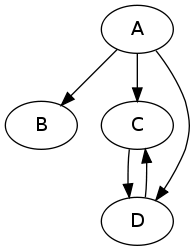
\includegraphics[width=1.4in]{figures/g1}
  \caption{Példa mérésből előálló gráf}
  \label{fig:g1}
\end{figure}
    
    \subsection{Megjelenítés}
    A feldolgozott adatok célja, hogy a karbantartó számára világossá tegye, hogy előfordulhat-e holtpont a mért alkalmazásban (azaz van-e két olyan szál, ami azonos erőforrásokon különböző zárolási sorrendet alkalmaz) és ha van, akkor segítse a karbantartó számára a problémás programrészek azonosítását. Ezen céloknak megfelelően a megjelenítés két részre oszlik.
    
    Egyrészről az alkalmazás biztosít egy gráfot (lásd~\ref{fig:g1}. ábra), mely az erőforrások zárolásának sorrendjét ábrázolja. 
    \begin{description}
        \item[Állítás:]Amennyiben a létrejövő gráf egy fa, a vizsgált erőforrások kölcsönös kizárást okozó zárolások nem juttatják holtpontra a mért alkalmazást.
        \item[Bizonyítás:]Indirekt módon. Tegyük fel, hogy az alkalmazást lemértük, nem jutott holtpontra, a mérés eredményeképpen előálló gráf egy fa és megfelelő időzítés esetén mégis előfordulhat holtpont. A holtpont kialakulásának feltétele az egymásra várás, vagyis T1 szál zárolta A erőforrást és vár B-re míg T2 szál zárolta B erőforrást és vár A-ra. Mivel más időzítési paraméterek mellett ez a két szál nem jutott holtpontra a mérés folyamán és sikeresen zárolták az erőforrásokat, az eredménygráf definíciója miatt A és B erőforrást reprezentáló csúcsok megjelennek és köztük irányított út található, tehát a gráfban kör van, tehát a gráf nem fa, így ellentmondásra jutunk.
    \end{description}
%    
    A felhasználó a mérés után ellenőrzi a gráfot; amennyiben az fa, az alkalmazás a fenti állításnak megfelelően a mért lefutás folyamán semmilyen időzítési paraméterek mellett nem futhat holtpontra, tehát nincs további módosításra szükség. Ha az eredménygráf nem fa, azaz tartalmaz irányított kört, akkor fennáll a holtpont előfordulásának veszélye, további vizsgálatra van szükség.
    
    Az érintett erőforrások vizsgálatát segíti a megjelenítést végző felület másik része. Az egyes erőforrásokat azonosító alapján -- mely megjelenik a gráf csúcsain -- kereshetjük ki a gyűjtött adatok közül, így képet kapva arról, hogy mely metódusok mentén történtek az egyes zárolások. A különböző zárolási hierarchiákat elemezve a karbantartó megállapíthatja, hogy melyik szál zársorrendje tekinthető \emph{hibásnak}, lokalizálva ezzel a módosítandó kódrészletet.
    
    \section{Implementáció}
    Az előzőekben a motivációra adott absztrakt választ részleteztem, kitérve a megoldás helyességének bizonyítására és értelmezésére, szorítkozva a feltétlenül szükséges logikai komponensekre, eltekintve az implementációs részletektől ott, ahol ez lehetséges volt. A következőkben az elkészített \emph{deadlockHunter} programot ismertetem először architekturális szinten, majd végigmegyek az egyes komponensek implementációs részletein, külön kiemelve a felmerülő kihívásokra adott válaszokat.
    
    \subsection{Architektúra}
    A fent specifikált alkalmazás megvalósítása architekturális szempontból két fő részt tesz szükségessé; Egy adatgyűjtésért és egy megjelenítésért felelős komponenst. A \emph{deadlockHunter} programban ez egy könyvtár (shared object) és egy bináris állomány formájában realizálódik. Az implementáció érdekessége, hogy a két komponens programkódja túlnyomó részben megegyezik. A \ref{fig:architecture}. ábra szemlélteti a komponensek kommunikációját.
    
\begin{figure}[ht!]
  \centering
    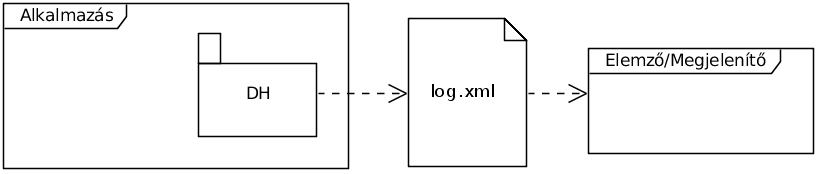
\includegraphics[width=5.4in]{figures/arch}
  \caption{Mérés komponenseinek lehetséges elrendezése}
  \label{fig:architecture}
\end{figure}    
%    
    A mérést végző komponens a gyűjtött adatokat vagy egy \texttt{XML} dokumentumba sorosítja, vagy Google Protocol Buffer\footnote{Google Protocol Buffer: https://developers.google.com/protocol-buffers} formátumba menti. A kinyert dokumentumot a megjelenítő komponens beolvassa és azokból egy gráfot készít valamint egy kereső felületet biztosít. A továbbiakban a két komponens jellemző részeit mutatom be röviden.
    
    \subsubsection{Google Protocol Buffer}
    Az \texttt{XML} formátum előnye, hogy karakteres természetéből adódóan ember számára is könnyen olvasható és kereshető, valamint gépi feldolgozása is egyszerű is rengeteg környezetben támogatott -- natív módon vagy könyvtárakon keresztül. Hátránya az \texttt{XML} formátumnak, hogy a dokumentum mérete a reprezentált információhoz képest nagyon nagy, amit körülményes tárolni és lassú beolvasni.
    
    A Google Protocol Buffer előnyei és hátrányai pont fordítottak. Azonos adatmennyiség sorosítás után sokkal kisebb méretű, mint \texttt{XML} esetében, a sorosított állomány beolvasása gyorsabb, viszont maga az állomány emberi olvasó számára értelmezhetetlen és az feldolgozás különböző platformokon külön támogatást és karbantartást igényel. Mivel jelen környezetben a kis méret és gyors feldolgozás abszolút prioritást élvez, a Protocol Buffer támogatás megjelenése után az \texttt{XML} formátum csupán tesztelési és kompatibilitási okokból van jelen a rendszerben.
    
    \subsection{Adatgyűjtés}
    Az adatgyűjtést úgy kellett megvalósítani, hogy a \emph{GlobalContractor} alkalmazásba könnyen integrálható legyen. A kódon végzett előzetes vizsgálat során kiderült, hogy minden kérdéses erőforrás -- többnyire rekurzív mutexek -- preprocesszor makrók egy szűk halmazának segítségével van zárolva és felszabadítva, a következő két idióma egyikével:
    
    \begin{description}
        \item[Guard idiom:] A makró egy osztályt példányosít a stacken. A konstruktor zárolja a megadott erőforrást, a blokk végére érve a stack lebontásakor pedig a destruktor felszabadítja azt.
        \item[Acquire/Release idiom:] Külön makrók állnak rendelkezésre az erőforrás zárolására és felszabadítására, melyek az átadott címen található struktúrán hívnak előre definiált metódusokat (\texttt{acquire()} és \texttt{release()}).
    \end{description}
%    
    Láthatóan mindkét megoldás könnyen kibővíthető úgy, hogy a zárolás \emph{és} felszabadítás tényét egy külső megfigyelő felé jelezze, anélkül, hogy a makródefinícióktól eltekintve a mért rendszeren bármilyen változtatást kéne eszközölni. Az első idióma esetén egy további osztály példányosítása, a második esetben egy-egy metódus meghívása elegendő.
    
    A makrók újradefiniálását egy fordítási időben állítható kapcsolóhoz köthetjük, így az alkalmazás futásidejű terhelést kizárólag a mérés során szenved el, egyéb esetekben a teljesítmény a módosítatlan változattal megegyezik (mivel ugyan az a programkód kerül fordításra).

\medskip    
\lstset{
    basicstyle=\footnotesize\ttfamily
}    
    \lstinputlisting[language=C++]{figures/macro.cpp}
\medskip

\noindent    
Ezeket a jelzéseket fogadja a mérés során az alkalmazáshoz linkelt könyvtár. Minden szál szálspecifikus tárában (\emph{thread local storage}) elérhető egy egyke mintát követő (\emph{singleton}) osztály példánya, ami a jelzéseket tárolja. A szálspecifikus tároló használatának előnye, hogy az események regisztrálása során a versenyhelyzetek figyelmen kívül hagyhatóak (mivel minden szál saját memóriaterületét módosítja).
    
    Az egyes lokális tárolókat egy globális tároló fogja össze. Elsődleges feladata a mérés végén a gyűjtött adatok sorosítása és fájlba írása. Ezen globális példány felületén keresztül szükség esetén -- még a mérés futása közben is -- diagnosztikai információkhoz juthatunk (lásd Megjelenítés) valamint átmenetileg felfüggeszthetjük vagy újraindíthatjuk az adatgyűjtést.
    
    A \emph{GlobalContractor} alkalmazás esetében a mérés vezérlése egy adminisztrációs felületbe integrálódott.
    
    \subsection{Megjelenítés}
    A mérési eredmények analizálása és vizualizációja két különböző felületen keresztül történhet. Hagyományos parancssoros, valamint egy böngészőből elérhető grafikus felület áll rendelkezésre.
    
    Bármely klienst is válasszuk, a megjelenítés elsődleges feladata a mérés során előzőleg sorosított adatok beolvasása és értelmezése. A program a feldolgozott adatokból egy gráfot épít (az erőforrások azonosítására a memóriacíme szolgál), amiből egy \emph{Graphviz\footnote{Graphviz: gráf vizualizációs szoftver, http://www.graphviz.org/} .dot\footnote{DOT leírónyelv: http://www.graphviz.org/doc/info/lang.html}} formátumú struktúrát készít, ami alapján a \emph{Graphviz} program a gráfot ábrázoló képfájlokat képes előállítani. A program által biztosított formátumok közül érdemes az \texttt{svg} formátumot választani, és azt Mozilla Firefox böngészővel megtekinteni. Bármely más tesztelt kombináció (megjelenítés: Mozilla Firefox, Google Chrome, Microsoft Internet Explorer, Windows Image and Fax Viewer; formátumok: jpg, png, svg) elfogadhatatlan hibákat okozott a megjelenítésben, a képfájlok szokatlanul nagy mérete miatt (pl.: $20.000 * 5000$ pixel). A gráf egyes csúcsain megjelenő feliratok a csúcs által reprezentált erőforrást definiáló osztály neve található -- amit a program a kapcsolódó fájl neve alapján tippel meg -- egy egyedi azonosítóval kiegészítve, pl.: \texttt{ModelProxy.23}. Az osztály név megjelenítésére azért esett a választás, hogy a program futása a tapasztalt karbantartó számára könnyen követhető legyen. Az egyedi azonosítóra az egyes osztályok különböző példányaiban definiált -- különböző -- erőforrások megkülönböztetése miatt van szükség. A gráf élei szálanként különböző színnel vannak színezve, a színek és szálazonosítók összerendelése táblázatban jelenik meg a képen.
    
    \subsubsection{Parancssoros felület}
    
    A parancssoros felület a kötelező feladatain túl képes a kimeneti formátumok között konvertálni, valamint egy keresőfelületet biztosít, ami a gráfon megjelenített nevek alapján keres az elemzett adatok között, és megjeleníti a keresett erőforrásra jellemző zárolásokat és környezetüket, szálanként csoportosítva (\ref{fig:trace}. ábra). A szálak azonosítása platformfüggő. Linux platformon a szálhoz rendelt \texttt{LWP} jelenik meg. Ennek előnye, hogy a \emph{gdb} program ugyanezt az azonosítót használja, így -- például -- egy coredump elemzése során az egyes szálak könnyen azonosíthatóak.
    
    Az egyes események szöveges reprezentációja egy formátumsztring megadásával konfigurálható. A megjeleníthető mezők a következőek:

\begin{description}
    \item[\%t] Esemény típusa (zárolás vagy felszabadítás)
    \item[\%f] Eseményt kiváltó metódus neve (GCC fordító használata esetén a \\ \texttt{\_\_PRETTY\_FUNC\_\_} kiegészítés használatával)
    \item[\%F] Kiváltó utasítást tartalmazó fájl neve
    \item[\%l] Kiváltó utasítást tartalmazó sor száma
    \item[\%a] Erőforrás memóriacíme
\end{description}

\noindent     
Az egyes mezők tetszőlegesen kombinálhatóak és kiegészíthetőek más karakterekkel.
    
\begin{figure}[ht!]
    \noindent
    \texttt{Thread \#12345 \\
    \\
    > lockFirst() (App.cc:186) \\
    \hspace*{8pt}    > lockSecond() (App.cc:219) [*]\\
    \hspace*{8pt}    < lockSecond() (App.cc:219) [*]\\    
    < lockFirst() (App.cc:186) \\
    \\
    Thread \#54321 \\
    \\
    > lockSecond() (App.cc:219) [*]\\
    \hspace*{8pt}    > lockFirst() (App.cc:186) \\
    \hspace*{8pt}    < lockFirst() (App.cc:186) \\
    < lockSecond() (App.cc:219) [*]\\
    }
  \caption{Keresés eredménye (példa). A *-al jelölt sorok a keresett erőforrásra vonatkozó események}
  \label{fig:trace}
\end{figure}

    \subsubsection{Grafikus felület}
    A parancssori felület megvalósítása egyszerű, a működése a lehető leggyorsabb, keresztplatformos megoldás, viszont rendelkezik néhány komoly hátránnyal is: a platformfüggetlen folyamkezlés miatt nem támogatja a kurzorbillentyűk kezelését, az automatikus parancs kiegészítést, valamint a használata nem intuitív. A problémák megoldása végett elkészítettem egy grafikus felületet, ami böngészőből érhető el.
    
    A működéshez szükség volt egy http szerverre, ami képes kommunikálni a C++ kódbázissal, elérhető a vállalati környezetben, pehelysúlyú és egyszerűen integrálható. A számbavett alternatívák a következőek:
    
\begin{description}
    \item[Mongoose:\footnotemark] \footnotetext{C++ nyelvű webszerver: https://github.com/valenok/mongoose}Kis méretű, egyszerű C++ szoftver, ami így nagyszerű választás lenne, de sajnos nem elérhető a vállalton belül.
    \item[Twisted:\footnotemark] \footnotetext{Python nyelvű esemény orientált hálózati motor: http://twistedmatrix.com/} Kiforrott, stabil szoftver, szimpatikus scriptnyelv; viszont nem találtam olyan Python/C++ interoperabilitási lehetőséget, ami megfelelt volna a követelményeknek.
    \item[Node.js:\footnotemark] \footnotetext{Javascript nyelvű hálózati platform: http://nodejs.org/} A követelményeket legnagyobb részben kielégíti és volt már tapasztalatom a szükséges felhasználási móddal. A Javascript/C++ integráció nem triviális és nagyon törékeny, lásd később.
   
\end{description}
%    
    A fentiek alapján a választás a Node.js-re esett. A Javascript/C++ kommunikáció megvalósítása végett készítettem egy Node.js \emph{addont}, ami a beérkező kéréseket továbbítja a C++ komponensnek, a választ pedig Javascript objektumok formájában teszi elérhetővé. Az integráció a Node.js által használt Google V8 Javascript motoron\footnote{Google V8 Javascript motor: http://code.google.com/p/v8/} alapul.
   
    Ezentúl írtam egy Node.js szerver programot Javascript nyelven, ami kiszolgálja az -- automatikusan elkészített, -- a mérést reprezentáló gráfot, lehetővé teszi a zárolási események kényelmes keresését, a szálak aggregált információinak megtekintését, valamint biztosít egy \emph{intelligens trace} funkciót.
    
    A keresési kifejezésre illeszkedő rögzített eseményeket listázó oldalon megjelenő kontextusok sora adott esetben hosszúra nyúlhat, és dacára minden optimalizációnak, többnyire egy erőforrásra vonatkozóan hasonló részleteket mutat, amelyek közül körülményes kikeresni az érdekes mintákat. A leggyakoribb feladat olyan minták keresése, ahol két erőforrás mindkét lehetséges sorrendben lefoglalásra kerül. A kérdéses erőforrások azonosítása lehetővé válik az eredménygráf vizsgálatával. A körök azonosításnak lehetőségét Tarjan erősen összefüggő komponensek algoritmusa és egy saját rekurzív konstrukció biztosítja. Az \emph{Autotrace} funkció az így kapott és érdekesnek ítélt, konfliktusos szálak releváns erőforrás kontextusait listázza.
    
    A felület használatához el kell indítani egy lokális Node.js szervert (\texttt{\$ node server.js}), ezután a konzolon megjelenő címen az alkalmazás elérhető. Az eredmények analizálása során a böngészett tartalmat egyértelműen azonosítja az URL-je, valamint egyes -- érdekesnek tartott -- részek külön meg is jelölhetőek, mely jelölések tükröződnek az URL-ben; így a karbantartó a fontos eredményeket egyszerűen meg tudja osztani kollégáival a linket továbbküldve. A felület funkcionalitásáért jQuery\footnote{jQuery: kliens oldalra szánt Javascript keretrendszer: http://jquery.com/}, az igényes megjelenéséért Twitter Bootstrap\footnote{Twitter Bootsrap frontend keretrendszer: http://twitter.github.com/bootstrap/} keretrendszerek felelnek.
    
    Az így kapott felület intuitív, valamint az eléréséhez csupán egy böngészőre van szükség. A megoldás hátránya, hogy a Javascript/C++ átmenetért felelős illesztő komponens lefordításához rendelkeznünk kell a megfelelő Node.js könyvtárakkal (\emph{shared object}), amiket ugyanazzal a fordítóval lettek fordítva.

    \section{Optimalizálás}
    A \emph{deadlockHunter} a fent leírt formában funkcionálisan késznek tekinthető, azonban használhatóság téren a gyakorlatban kívánnivalókat hagy maga után. A kezdeti tesztelések megmutatták, hogy egy igazán komplex alkalmazás hosszas mérése komoly teljesítménybeli problémákat okozhat. A konkrét problémákat a következő alfejezetekben ismertetem a megoldásaikkal együtt. Amikor ezek a problémák felmerültek, a kiutat nem a kód mikrooptimalizálásában kerestem, -- egy-egy gépi utasítás megspórolása itt-ott nem segített volna -- hanem az adatstruktúrák és algoritmusok javításában. Ennek megfelelően aprólékos kódoptimalizálásra nem került sor, mivel nem volt rá szükség.
    
    \subsection{Az adatgyűjtés optimalizálása}
    
Az egyik problémát a mérés folyamán az események válogatás nélküli regisztrálása jelentette. A mért alkalmazásban gyakran előfordult a következő minta: Egy nagy elemszámú listán iterált, minden elem feldolgozása előtt az elemet zárolta egy megfelelő mutexen keresztül, majd a feldolgozás végeztével a zárat elengedte. Ez sok esemény bejegyzését jelentette. Mivel ezeket az iterációkat az alkalmazás minden gerjesztés mellőzése esetén, "üresjáratban" is folytatta, a tárolt események száma nagyon gyorsan növekedett, hamar túllépve a rendelkezésre álló memóriát (A tesztkörnyezetben 16 GB-ot).

    A triviális megoldása a problémának, hogy a tárolt események számának függvényében azokat időnként a háttértárra mentjük és a memóriából eltávolítjuk. Ennek a megközelítésnek több hátulütője is van: Továbbra is rengeteg eseménnyel kell majd foglalkozi a megjelenítés során, ami ott újabb teljesítményproblémákhoz vezethet, a hatalmas kimeneti fájlok kezelése nehézkes és archiválásuk költséges valamint a folyamatos fájlműveletek feleslegesen lassítják a mérést.
    
    Egy jobb megoldáshoz jutunk, ha a fent említett mintát figyeljük meg. A ciklus ismételt futtatása újból és újból ugyan azokat az eseménysorokat eredményezi. Egyszerűen adódna, hogy akkor ezeket az ismétléseket csoportosítsuk, és spóroljuk meg például az ismétlődő stringek tárolását egy string cache használatával. Ez egy életképes elgondolás, azonban az eseménycsoportok összehasonlítása újabb felismeréshez vezet el: Kizárólag az időzítési paramétereikben különböznek, vagyis egy olyan jellemzőben, amit szándékosan nem veszünk figyelembe mivel a gráfalkotás során ez az információ eldobásra kerül. Tehát az egyes eseménycsoportok közül egy tetszőleges kivételével a többi eldobható, anélkül, hogy veszítenénk a mérés pontosságából.
    
    Ennek megfelelően az eseményeket regisztráló komponens a következő képpen változik:
    
    \begin{enumerate}
        \item Kezdetben egy üres csoportlistával és egy üres átmeneti listával jön létre
        \item A beérkező eseményeket az átmeneti listában rögzíti
        \item A csoport végén az átmeneti listát összehasonlítja az összes eddigi csoporttal. Ha talál olyan csoportot, amely megegyező sorrendben tartalmaz az átmeneti csoportban található eseményekkel ekvivalens eseményeket, és csak azokat, akkor az átmeneti listát eldobja, és újat kezd. Egyébként az átmeneti listát elmenti új csoportként, és ezután üríti.
    \end{enumerate}
    
    Hogy a megoldás működhessen két fogalmat kell definiálni: Mikor van egy csoportnak vége, valamint mikor mondunk két eseményt ekvivalensnek. Mindkét fogalom nagyon komolyan befolyásolja a mérés kimenetelét, a definíciókat úgy határoztam meg, hogy azok segítsék a \emph{GlobalContractor} mérését. Más alkalmazás esetén előfordulhat, hogy egy alkalmasabb definíció található.
    
    A csoportok határának meghatározására a szál által zárva tartott erőforrások számát használtam fel. Ehez nyilván kell tartani a mérőszámot, ami konstans időben megtehető. Amennyiben a zárolt erőforrások száma elér egy előre meghatározott korlátot, az aktuális csoport lezárásra kerül. A korlátot alkalmasan kell megválasztani, a gyakori minták függvényében. A \emph{GlobalContractor} esetében ezt a korlátot a 0 szinten határoztam meg. Amennyiben egy szál elenged minden erőforrást, zárolódik az addigi tevékenysége. (Ez a választás elősegítette azt is, hogy a csoportok használata egy teljesen más helyzetben nyújtson segítséget) Ha előfordul, hogy egy szál futásának kezdetén magához ragad egy erőforrást, és azt hosszú időn keresztül nem engedi el, miközben sok különböző tevékenységet hajt végre -- sok eseményt generál -- akkor megfontolandó a korlát felemelése, hogy az így kialakuló nagyméretű csoportokat feldaraboljuk. Ennek ára van, 0-tól különböző korlát használata további óvintézkedéseket igényel, egy esetleges hibás mérést megelőzendő.
    
    Az egyes események közötti egyenlőség operátor definiálása során ugyancsak érdemes figyelembe venni az alkalmazás jellegzetességeit. Amennyiben ezt nem tesszük meg, a válasz triviálisan adódik: Két esemény megegyezik, ha minden róla tárolt információ megegyezik (pl.: fájl, sor és memóriacím). Ez a választás helyességét tekintve megfelelő, viszont a kritérium relaxálásával könnyebben feldolgozható eredményt kapunk. Bizonyos esetekben előfordulhat, hogy megengedhejük a memóriacím különbözőségét (és csak a fájlt valamint a sort ellenőrizzük). Ez a választás a legtöbb esetben nem helyes, viszont alkalmanként mégis jó és könnyen elemezhető gráfhoz vezet minket, amin jobban megfigyelhetőek az egyes zárolási minták.
    
    A \emph{GlobalContractor} esetében, más optimalizációk használata mellett a választás a fájl nevét, a forráskód sorszámát és az erőforrás memóriacímét figyelembe vevő egyenlőség operátorra esett.
    
    Az optimalizáció megvalósítását követően a mérőkóddal ellátott alkalmazás memóriahasználata alig tért el az alapértelmezett működés közben megfigyelhető igényektől, és üresjáratban semmilyen emelkedést nem mutatott, így teljes mértékben elérte célját.
    
    \subsection{Az adatgyűjtés optimalizálásának teljesítménymérése \textcolor{red}{TODO}}
    Ha sikerül hozzáférni az alkalmazáshoz, ide kerülhet egy grafikon és magyarázat a mérési eredményekről. %TODO
    
    \subsection{A megjelenítés optimalizálása}
    Egy kiterjedt teszt futtatása -- még a fenti optimalizáció figyelembe vételével is --nagyon sok regisztrált eseményhez vezet, ami a gráf reprezentációt áttekinthetetlenné teszi. A probléma forrása, hogy olyan események is megjelennek, amelyek nem vesznek részt holtpont kialakításában. Az ilyen eseményeket reprezentáló csúcsokat eltüntethetjük, ha az eredménygráf levél csúcsainak levágását addig ismételjük, amíg van ilyen csúcs.
    
    \begin{description}
        \item[Állítás:] A gráf leveleinek ismételt levágásával nem veszítünk el lehetséges holtpontra utaló mintát.
        \item[Bizonyítás:] Korábban beláttuk, hogy a gráf konstrukciója miatt csak akkor alakulhat ki holtpont az alkalmazásban, ha az irányított gráf nem fa, vagyis ha irányított kört tartalmaz. Tehát amíg nem vágunk le olyan csúcsot, ami egy irányított kör eleme, addig nem veszítünk el értékes információt sem. Mivel egy csúcs pontosan akkor levél, ha nincs belőle kimenő irányított él, ezért egy levél nem lehet irányított kör eleme, tehát elhagyható. Mivel az így keletkező gráf pontosan ugyan azt az értékes információt hordozza, mint az előző, a lépést megismételhetjük, egészen addig, amíg van levél csúcs.
        \item[Megjegyzés:] Ha az eredménygráf fa, az összes csúcsot eldobhatjuk és üres gráfot kapunk -- tehát holtpontra nincs lehetőség -- ami megfelel a korábbi állításnak.
    \end{description}
%    
    Az így kapott, jelentősen redukált méretű gráf sokkal könnyebben elemezhető, ám egy -- az előzőhöz nagyon hasonló -- ötlettel még több csúcsot hagyhatunk el.
    
    \begin{description}
        \item[Állítás:] A gráf gyökér csúcsainak ismételt levágásával nem veszítünk el lehetséges holtpontra utaló mintát.
        \item[Bizonyítás:] Az előző mintájára. Egy csúcs pontosan akkor gyökér, ha nem mutat rá irányított él, tehát nem mehet át rajta irányított kör, vagyis eldobható. Az értékes információ megmaradása miatt a lépés ismételhető, amíg van gyökér pont.
        \item[Megjegyzés:] Az előző módszerhez hasonlóan, csak ezt az eljárást alkalmazva pontosan akkor lesz a kimeneti gráf az üres gráf, ha a bemeneti gráf fa volt.
        \item[Megjegyzés 2:] A módszert alkalmazva a gráf elveszítheti összefüggőségét.
    \end{description}
%    
    A bemutatott két módszerrel transzformált gráf nagyságrendekkel kevesebb csúcsot tartalmazott a \emph{GlobalContractor} esetében és emberi vizsgálatra sokkal alkalmasabbnak bizonyult. Tekintve, hogy a fenti tételek szerint információt nem veszítettünk, az optimalizáció hasznosnak ítélhető.
    
    %\section{Felhasználói segédlet}
    %\subsection{Fejlett felhasználás}
    
    \section{Fejlesztési tervek}
    A \emph{deadlockHunter} jelen formájában használható és betölti a célját, viszont a fejlesztés és tesztelés során felmerültek további ötletek, melyek növelnék a felhasználóbarátságot vagy a project fejlődése miatt fontosak. Az örökös fejlődés igénye egy szoftver sajátja és szerves része, ezért ezen ötletek közül a következőkben ismertetem a legfontosabbakat.
    
    \subsection{Forráskód megnyitása}
    A project nem jöhetett volna létre a fejlesztés során használt számtalan nyílt forráskódú szoftver nélkül (pl.: Linux, GCC, Eclipse, git, boost, graphviz és mások), így egyértelmű a forrás megnyitásának motivációja, tekintve továbbá, hogy az eszköz általános célú, így más környezetben is hasznosnak bizonyulhat.
    
    A \emph{deadlockHunter} már nem tartalmaz \emph{proprietary} függőségekket, azokat lecseréltem funkcionálisan ekvivalens, nyílt forráskódú alternatíváikra. Az utolsó lépés, hogy a forráskód megnyitását a Morgan Stanley megfelelő testülete is jóváhagyja. Az erőfeszítés sikeressége egyelőre bizonytalan, de valószínűsíthető. Amennyiben az akció sikerrel jár, az eszköz szabadon elérhetővé tétele az eddigi gyakorlattól eltérő, egyedülálló esemény lesz a vállalat történetében, és remélhetőleg egy új irány kezdete.
    
    \subsection{Felhasználói dokumentáció készítése}
    Ha sikerül a forráskód megnyitása, szükségessé válik egy mindenki számára szabadon elérhető dokumentáció elkészítése is, mely tartalmazz felhasználói segédletet és integrátori útmutatót is. Mivel jelen dokumentum a teljesség igényével részletezi az alkalmazás fontos részeit, nem alkalmas a felhasználói dokumentáció szerep betöltésére.
    
    \subsection{Automatikus kiegészítés a keresőben}
    A grafikus felületet az egyszerűbb és kényelmesebb használat érdekében kell úgy továbbfejleszteni, hogy a keresőben megjelenjenek a lehetséges, illeszkedő keresőkifejezések, automatikus kiegészítés formájában. Ehhez meg kell teremteni a lehetőséget, hogy a C++ oldal kiajánlja a rendelkezésre álló opciókat.
    
    \subsection{Kódtisztítás}
    A C++ programkódon elvégzendő néhány apró, de átfogó változtatás:

    \begin{description}
        \item[Dokumentáció:] Ahol esetleg még hiányzik az API dokumentáció, ott azt el kell készíteni, valamint az összes API dokumentációt át kell nézni és az esetlegesen elavult részeket frissíteni kell. Ezután a forráskódból különálló dokumentációt kell generálni, az automatizmust rögzítve, megismételhető módon.
        
        \item[Projekt namespace:] Az integráció egyszerűsítése végett az összes komponenst egy közös \texttt{namespace} alá kell helyezni.
        
        \item[Guard macro nevek:] A fejléc fájlok \emph{guard macro}i jelenleg a következő formátumban vannak: \texttt{\_CLASSNAME\_H}. Ezt kell átalakítani úgy, hogy tükrözze a könyvtárstruktúrát.

    \end{description}


%\listoffigures\addcontentsline{toc}{chapter}{Ábrák jegyzéke}
%\listoftables\addcontentsline{toc}{chapter}{Táblázatok jegyzéke}

%----------------------------------------------------------------------------
\chapter*{Köszönetnyilvánítás}
\addcontentsline{toc}{chapter}{Köszönetnyilvánítás}
%----------------------------------------------------------------------------

Köszönetet mondok családomnak, hogy szeretettel viselték, amikor esténként munkából hazatérve ahelyett, hogy velük együtt -- családi körben -- töltöttem volna a vacsorát, szégyentelenül néhány diétás sonkás sajtos szalámis szendviccsel és egy liter tejjel elvonultam és számítógépem társaságában görnyedtem végig az estét, majd az éjszakát.

Köszönöm anyai nagymamámnak, hogy jelentős mennyiségű konverzibilis tárgyi eszközt bocsájtott rendelkezésemre -- az általa biztosított cukros kekszgolyók ATP-re konvertálása még a legsötétebb éjjeli órák idején is képes volt újabb (a felhasználások számával lineárisan növekvő konstanssal amortizált) 10 perc munkára elegendő energiát biztosítani.

Köszönöm apai nagymamámnak, hogy házi baracklekvárával és paradicsomlevével felvidította a reggeli ébredés pillanatait -- ekkor mindig feledni tudtam a hátalévő fejezetek számát. Hálás vagyok neki, hogy szívén viseli szakbarbarizmusom előrehaladott állapotát és mindig továbbküldi a kulturális témájú zenés prezentációkat tartalmazó körleveleket -- bennem a fentebb stíl művelését elősegítendő.

Köszönöm apai nagyapámnak, hogy már akkor bevezetett a tranzisztorok varázslatos világába, amikor még az Ohm törvényben található betűket sem ismertem -- ha nincs az ő szelíd, de határozott gondoskodása, amivel az egyetlen igaz életpálya felé terelt, most talán egy vidéki színjátszó szakkör felolvasópróbáján ülnék vagy egy székmentes keleti jellegű pesti teázó padlóján próbálnék egy alárendelő módon többszörösen bővített, didaktikus elemekkel gondosan körülvett mondatot még kacifántosabbá tenni.

Köszönöm anyai nagyapámnak, hogy megmutatta, hogyan kell nyulat nyúzni, kulcsot másolni és hogy milyen szép a kilátás a kilencemeletes tetejéről. Biztos vagyok benne, hogy születésnapi köszöntései nagymértékben inspiráltak.

Köszönöm dédszüleimnek -- különösen anyai-apai dédanyámnak -- hogy folyamatos lelki támogatást nyújtottak a legelkeseredettebb időkben is. Dédi! Tudom, hogy megígértem, hogy idős korodban majd gondodat viselem. Nem felejtettelek el, mégha ritkán beszélünk is! Még van egy-két elintézni valóm, de hamarosan találkozunk.

Köszönöm barátaimnak, hogy szeretnek és elfogadnak, valamint biztosítanak munkám nélkülözhetetlenségéről még akkor is, amikor a dolgozatom címének részletezése közben tekintetük kissé ködössé válik. Külön köszönöm, hogy egészségemmel nem törődve születésnapom alkalmából megajándékoztak 5 teljes rúd $\int_{-\infty}^\infty f(x)\ e^{- 2\pi i x \xi}\,dx$ típusú csokis keksszel. Ezek majdnem végig kitartottak, csupán a C++ szabvány olvasása közben meginduló kegyetlen ostromnak nem tudtak ellenállni. Nélkületek nem sikerült volna.

Köszönöm a Morgan Stanley Magyarország Elemző Kft-nek, hogy finanszírozta a dolgozat alapját adó program elkészítését és megengedte a fejlesztés során összegyűjtött tapasztalatok és kutatási eredmények publikálását. Szívet melengető érzés, hogy három manager is elolvasta a releváns fejezeteket, tőlük ezúton kérek elnézést, én magamtól soha, (soha!) nem írnék ennyit.

A dolgozat nem jöhetett volna létre számos nagyszerű -- többnyire nyílt forráskódú -- program nélkül. Ezek közül a teljesség igénye nélkül néhány: Linux, GCC, Git, \LaTeX, Gnome, vim, Firefox. Köszönet a fejlesztőknek és tamogatóknak!

\vfill
\begin{center}
\emph{Mondottam, ember, küzdj és bízva bízzál!}
\end{center}
\thispagestyle{empty}


\addcontentsline{toc}{chapter}{Irodalomjegyzék}
\bibliography{mybib}
%\cleardoublepage\phantomsection
\bibliographystyle{abstract}

%\include{appendices}

\label{page:last}
\end{document}
